\chapter{Foundation of Logical Normal Form Networks}\label{C:foundation-of-lnfns}
This chapter motivates the concept of Logical Normal Form Networks (LNFNs) along with re-deriving them in terms of Noisy Neurons. The training of LNFNs is discussed in the form of deriving a weight initialization method, choosing a algorithm to propagate gradients and justifying a choice of mini-batch size. LNFNs are also compared against Multi-Layer Perceptron Networks (MLPNs) using randomly generated truth tables as the data sets.\\

Consider the set of binary classification problems which have boolean inputs. Consider some problem $p$ in this set, with $X_p$ and $Y_p$ being the examples and targets retrospectively. Let $B_p$ be the set of all boolean functions which take an $x \in X_p$ and take it to either a 1 or 0. Then finding the optimal boolean function to solve the problem $p$ corresponds to expression \ref{equ:arg-max-boolean-function} which is simply the function $f$ with the smallest cross entropy loss.

\begin{equation}
\label{equ:arg-max-boolean-function}
\begin{aligned}
& \underset{f \in B_p}{\text{arg min}}
& & -\sum_{0 \leq i \leq |X_p|} (Y_{p_i} \cdot \log f(X_{p_i})) + ((1 - Y_{p_i}) \cdot \log(1 - f(X_{p_i})))  \\
\end{aligned}
\end{equation}

How might a interpretable network architecture that can learn these functions be constructed? The following facts will be helpful, any boolean function has a unique Conjunctive and Disjunctive Normal Form (CNF \& DNF), both the CNF and DNF are described by the boolean operations NOT, OR and AND, in a CNF or DNF a not can only occur on a literal and the maximum number of clauses in a CNF or DNF is $2^n$ where n is th number of inputs.\\

One option is to use a standard Multi-Layer Perceptron Network (MLPN). MLPNs have been shown to be universal function approximators but are not interpretable. Learning the CNF or DNF of the optimal function is an equivalent problem. For now consider the problem of learning the CNF. This can be done with hidden layer of size $k$ and an output layer with a single neuron. The hidden neurons only need to perform the OR operation on a subset of inputs. The output layer only need perform an AND of a subset of the hidden neurons.\\

Using Noisy-OR and Noisy-AND (See Section \ref{sec:background-noisy-neurons}) such a network can be constructed. Noisy neurons can not compute the not of inputs so the input layer must be modified to include the negation of each input. Figure \ref{fig:cnf-network-structure} is the structure that has been derived.

\begin{figure}[H]
	\centering
	\begin{minipage}[b]{0.6\textwidth}
		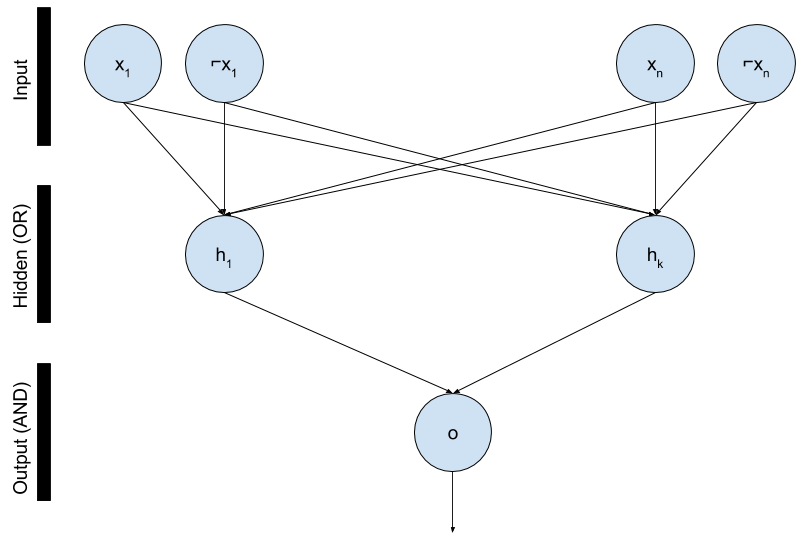
\includegraphics[width=\textwidth]{CNF-Network-Structure.png}
		\caption{Network Architecture for Learning CNF}
		\label{fig:cnf-network-structure}
	\end{minipage}
	\hfill
\end{figure}

By the same logic a network architecture for learning the DNF can be derived, the hidden layer consists of ANDs and the output of a single OR. These networks for learning CNF and DNF formulae are a new derivation of Logical Normal Form Networks (LNFNs) \cite{herrmann1996backpropagation}, the difference being Noisy neurons are used instead of the previously derived Conjunctive and Disjunctive neurons. Definitions of CNF Networks, DNF Networks and LNFNs are now given.

\theoremstyle{definition}
\begin{definition} \label{def:cnf-network}
A \textbf{CNF-Network} is a three layer network where neurons in the hidden layer consist solely of Noisy-OR's and the output layer is a single Noisy-AND. 
\end{definition}

\theoremstyle{definition}
\begin{definition} \label{def:dnf-network}
A \textbf{DNF-Network} is a three layer network where neurons in the hidden layer consist solely of Noisy-AND's and the output layer is a single Noisy-OR. 
\end{definition}

\theoremstyle{definition}
\begin{definition} \label{def:lnfn}
A \textbf{LNF-Network} is a DNF or CNF Network
\end{definition}

It must also be determined how many hidden units the LNFN will have, it is known that $2^n$, n being the number of atoms, is an upper bound on the number of clauses needed in a CNF and DNF formula (see Theorem \ref{thm:max-clause-cnfdnf}).

\begin{theorem}
Let T be the complete truth table for the boolean formula B. Let L be an LNFN, if L has $2^n$ hidden units then there always exists a set of weights for L which correctly classifies any assignment of truth values to atoms.
\label{thm:upper-bound-hidden-units}
\end{theorem}

\begin{proof}
Let T be the truth table for a boolean function B. The atoms of B are $x_1, ..., x_n$. T has exactly $2^n$ rows. Construct an LNFN, L, in the following manner. L has $2^n$ hidden units and by definition L has one output unit. The inputs to L are $i_1, ..., i_{2n}$ where $i_1, i_2$ represent $x_1, \lnot x_1$ and so on. Let $\epsilon_b = 1$ for every neuron.\\

Let $h_k$ denote hidden unit k. $h_k$ has the weights $\epsilon_{k,1}, ..., \epsilon_{k,2n}$, where $\epsilon_{k, m}$ represents input $i_m$'s relevance to the output of $h_k$. Similarly the output unit $o$ has weights $\mu_1, .., \mu_{2^n}$ where $\mu_m$ represents the relevance of $h_m$ to the output of $o$.\\

Assume L is a DNF Network. Starting from row one of the table T, to row $2^n$. If row $a$ corresponds to False then set $\mu_a = 1$ (i.e. hidden node $a$ is irrelevant), otherwise the row corresponds to True, then $\mu_a = Z$, where Z is a value close to 0 (any weight for a Noisy neuron cant be exactly 0). For each $\epsilon_{a, m}$ if the corresponding literal occurs in row $a$ of the truth table then $\epsilon_{a, m} = Z$ other wise $\epsilon_{a, m} = 1$.\\

\textbf{Claim:} For some assignment to the atoms of B, $x_1 = v_1, ..., x_n = v_n$ where $v_i \in \{0, 1\}$. Then $L(i_1, ..., i_{2n}) = B(x_1, ..., x_n)$.\\

Assume $B(x_1, ..., x_n) = 1$ for the assignment $x_1 = v_1, ..., x_n = v_n$ corresponding to row $a$ of T. Then if $i_k$ is not considered in row $a$ then $\epsilon_{a,k} = 1$ and if it is present then $i_k = 1$. The output of $h_a$ is given by 

\begin{align*}
&= \prod \epsilon_{a, m}^{1 - i_m}\\
&= Z^{\sum_{i_k = 1}(1 - i_k)}\\
&= Z^0
\end{align*}
Demonstrating that  $\lim_{Z \to 0} Out(h_a) = \lim_{Z \to 0} Z^0 = 1$. Consider the activation of $o$, it is known that $\mu_a = Z$ consequently $\lim_{Z \to 0} \mu_a^{h_a} = \lim_{Z \to 0} Z^1 = 0$, therefore

\begin{align}
\lim_{Z \to 0} Out(o) &= 1 - \prod_{m=1}^{2^n} \mu_m ^{h_m}\\
&= 1 - 0 = 1
\end{align} 

Therefore $L(i_1, ..., i_{2n}) = 1$. Alternatively if $B(x_1, ..., x_n) = 0$ then no hidden neuron will have activation $1$, this can be demonstrated by considering that any relevant neuron (i.e. corresponding $\mu \neq 1$) will have some input weight pair of $i_m$ $\epsilon_m$ such that $\epsilon_m^{i_m} = 0$. Consequently it can be said that for all $m$ $\mu_m^{h_m} = \mu_m^{0} = 1$, therefore the output unit will give $0$, as required.

Now assume that L is a CNF Network. The weights can be assigned in the same manner as before, except rather than considering the rows that correspond to True the negation of the rows corresponding to False are used. If a row $a$ corresponds to True then $\mu_a = 1$, otherwise $\mu_a = Z$ and for any literal present in the row then the input to L which corresponds to the negated literal has weight $Z$, all other weights are $1$.\\

\textbf{Claim:} For some assignment to the atoms of B, $x_1 = v_1, ..., x_n = v_n$ where $v_i \in \{0, 1\}$. Then $L(i_1, ..., i_{2n}) = B(x_1, ..., x_n)$.\\

In this configuration it must be shown that every hidden neuron fires when the network is presented with a variable assignment which corresponds to True and there is always at least one neuron which does not fire when the assignment corresponds to False. Assume for a contradiction that for a given assignment $B(x_1, ..., x_n) = 1$ but $L(i_1, ..., i_{2n}) = 0$. Then there is at least one hidden neuron which does not fire. Let $h_a$ be such a neuron. Consequently for any input weight combination which is relevant $\epsilon_{a,m}^{i_m} = 1$, so $i_m = 0$ for any relevant input. Let $i_{r_1}, ..., i_{r_k}$ be the relevant inputs then $i_{r_1} \lor ... \lor i_{r_k} = False$, so $\lnot(\lnot i_{r_1} \land ... \land \lnot i_{r_k}) = False$, a contradiction as then $B(x_1, ..., x_n)$ would be False.

Now assume for a contradiction $B(x_1, ..., x_n) = 0$ but $L(i_1, ..., i_{2n}) = 1$. Then there exists some $h_a$ with output $1$ where it should be $0$. Consequently there exists at least one input/weight pair with $\epsilon_{a,m}^{i_m} = 1$ that should be $0$. Let $i_{r_1}, ..., i_{r_k}$ be all the relevant inputs, at least one relevant input is present $i_r$. Consequently $i_{r_1} \lor ... \lor i_{r_k} = True$, therefore $\lnot(\lnot i_{r_1} \land ... \land \lnot i_{r_k}) = True$, a contradiction as then $B(x_1, ..., x_n)$ is True.\\
\end{proof}

Theorem \ref{thm:upper-bound-hidden-units} provides justification for using $2^n$ hidden units, it guarantees that there at least exists an assignment of weights yielding a network that can correctly classify each item in the truth table.

\section{Noisy Gate Parametrisation} \label{sec:real-noisy-parametrisation}
The parametrisation of Noisy gates require weight clipping, an expensive operation. A new parametrisation is derived that implicitly clips the weights. Consider that $\epsilon \in (0, 1]$, therefore let $\epsilon_i = \sigma(w_i)$, these $w_i$'s can be trained without any clipping, after training the original $\epsilon_i$'s can be recovered.\\

Now these weights must be substituted into the Noisy activation. Consider the Noisy-OR activation.

\begin{align*}
a_{or}(X) &= 1 - \prod^p_{i=1}(\epsilon_i^{x_i}) \cdot \epsilon_b\\
&= 1 - \prod^p_{i=1}(\sigma(w_i)^{x_i}) \cdot \sigma(b)\\
&= 1 - \prod^p_{i=1}((\frac{1}{1 + e^{-w_i}})^{x_i}) \cdot \frac{1}{1 + e^{-b}}\\
&= 1 - \prod^p_{i=1}((1 + e^{-w_i})^{-x_i}) \cdot (1 + e^{-w_i})^{-1}\\
&= 1 - e^{\sum^p_{i=1} -x_i \cdot ln(1 + e^{-w_i}) - ln(1 + e^{-b})} \\
&Let\ w_i^{'} = ln(1 + e^{-w_i}),\ b^{'} = ln(1 + e^{-b})\\
&= 1 - e^{-(W^{'} \cdot X + b^{'})}
\end{align*}

From a similar derivation we get the activation for a Noisy-AND.

\begin{align*}
a_{and}(X) &= \prod_{p}^{i=1} (\epsilon_i^{1 - x_i}) \cdot \epsilon_b\\
&= \prod_{p}^{i=1} (\sigma(w_i)^{1 - x_i}) \cdot \sigma(w_b)\\
&= e^{\sum^p_{i=1} -(1 - x_i) \cdot ln(1 + e^{-w_i}) - ln(1 + e^{-b})} \\
&= e^{-(W^{'} \cdot (1 - X) + b^{'})}
\end{align*}

Concisely giving equations \ref{equ:real-noisy-and-activation}, \ref{equ:real-noisy-or-activation}

\begin{align}
a_{and}(X) &= e^{-(W^{'} \cdot (1 - X) + b^{'})} \label{equ:real-noisy-and-activation}\\
a_{or}(X)&= 1 - e^{-(W^{'} \cdot X + b^{'})} \label{equ:real-noisy-or-activation}
\end{align}

The function taking $w_i$ to $w_i^{'}$ is the soft ReLU function which is performing a soft clipping on the $w_i$'s. 

\section{Training LNF Networks}
Using equations \ref{equ:real-noisy-or-activation} and \ref{equ:real-noisy-and-activation} for the Noisy-OR, Noisy-AND activations retrospectively allows LNFNs to be trained without the need to clip the weights.\\

Before these networks can be trained a number of choices must be made. These are outlined in the list below.

\begin{enumerate}
	\item \textit{Weight Initialization:} A method for initializing the weights must be derived, \hl{if this is not carefully thought about then it could lead to poor training conditions.}
	\item \textit{Training Algorithm:} \hl{There exsists a number of different algorythms for propergating gradients}, one must be chosen based on the properties of these networks.
	\item \textit{Batch Size:} What size should each batch be when training these networks.
\end{enumerate}

\subsection{Weight Initialization}
The following section derives a method for initializing weights in an LNFN.

\paragraph{Deriving a Distribution For The Weights}
Before a weight initialization algorithm can be derived good learning conditions must be identified. Ideally the output of each neuron would be varied for each training example, i.e. $y \sim U(0,1)$. Each training example $X = \{x_1, ..., x_n\}$ has each component $x_i \in (0,1]$, it will be assumed that $x_i \sim U(0,1)$. If the input vectors and output of each neuron are both distributed $U(0,1)$ then the input to any layer is distributed $U(0,1)$, based on this fact it can be argued that the weight initialization is the same for both Noisy-OR and Noisy-AND. Recall the activations for Noisy neurons\\

\begin{align*}
a_{AND}(X) &= e^{-(w_1(1 - x_1) + ... + w_n(1 - x_n))}\\
a_{OR}(X) &= 1 - e^{-(w_1x_1 + ... + w_nx_n)}
\end{align*}

Consider a random variable $g$, if $g \sim U(0,1)$ then $1 - g \sim U(0,1)$ also holds. Consequently, if $x_i \sim U(0,1)$ then $1 - x_i ~ U(0,1)$, also $e^{-z} \sim U(0,1)$ then $1 - e^{-z} ~ U(0,1)$. It is therefore enough to consider $e^{-(w_1x_1 + ... + w_nx_n)}$ when deriving the initialization method for each $w_i$.\\

Strictly speaking each $w_i = \log(1 + e^{w^{'}_i})$ (as derived in Section \ref{sec:real-noisy-parametrisation}) however for the purposes of this initialisation derivation it will be assumed that $w_i \in (0 \infty]$.\\

Given that $y = e^{-z} ~ U(0,1)$, a first step is to determine the distribution of $z$.

\begin{theorem}
	If $y \sim U(0,1)$ and $y = e^{-z}$, then $z \sim exp(\lambda = 1)$
\end{theorem}
\begin{proof}
	Consider that $y = e^{-z}$ can be re written as $z = -\log(y)$.
	
	\begin{align*}
	F(z) &= P(Z < z)\\
	&= P(-\log(Y) < z)\\
	&= P(\frac{1}{Y} < e^{-z})\\
	&= P(Y \geq e^{-z})\\
	&= 1 - P(Y \leq e^{-z})\\
	&= 1 - \int_{0}^{e^{-z}} f(y) dy\\
	&= 1 - \int_{0}^{e^{-z}} 1 dy\\
	&= 1 - e^{-z}
	\end{align*}
	
	Therefore $F(z) = 1 - e^{-\lambda z}$ where $\lambda = 1$. Consequently $z \sim exp(\lambda = 1)$
\end{proof}

The problem has now been reduced to find how $w_i$ is distributed given that $z \sim exp(\lambda = 1)$ and $x_i \sim U(0,1)$. The approach taken is to find $E[w_i]$ and $var(w_i)$.

\begin{align*}
E[z] &= E[w_1x_1 + \cdot \cdot \cdot + w_nx_n]\\
&= E[w_1x_1] + \cdot \cdot \cdot + E[w_nx_n]\ (independence)\\
&= E[w_1]E[x_1] + \cdot \cdot \cdot + E[w_n]E[x_n]\\
&= n \cdot E[w_i]E[x_i]\ (i.i.d)\\
&= n \cdot E[w_i] \cdot \frac{1}{2}\\
1 &= \frac{n}{2} \cdot E[w_i]\\
E[w_i] &= \frac{2}{n}
\end{align*}

\begin{align*}
var(z) &= var(w_1x_1 + \cdot \cdot \cdot + w_nx_n)\\
&= var(w_1x_1) + \cdot \cdot \cdot + car(w_nx_n)\\
\end{align*}

\begin{align*}
var(w_ix_i) &= (E[w_i])^2var(x_i) + (E[x_i])^2var(w_i) + var(w_i)var(x_i)\\
&= \frac{4}{n^2} \cdot \frac{1}{2} + \frac{1}{4} \cdot var(w_i) + var(w_i) \cdot \frac{1}{12}\\
&= \frac{1}{3 n^2} + \frac{1}{3}var(w_i)
\end{align*}

Consequently the variance can be found by the following

\begin{align*}
1 &= n \cdot \big[\frac{1}{3 n^2} + \frac{1}{3}var(w_i)\big]\\
3 &= \frac{1}{n} + n \cdot var(w_i)\\
3n &= n^2 var(w_i)\\
var(w_i) &= \frac{3}{n}
\end{align*}

From the above arguments $E[w_i] = \frac{2}{n}$ and $var(w_i) = \frac{3}{n}$. These values need to be fitted to a distribution that weights can be sampled from. Based on our initial assumptions this distribution must also generate values in the interval $[0, \infty]$. There exists a number of different distributions which satisfy this constraint, for example Beta Prime, Log Normal, Poison. Based on experimental evidence the Log Normal distribution had the best results so for brevity only its derivation is included.

\paragraph{Fitting To Log Normal}

A LogNormal distribution has two parameters $\mu$ and $\sigma^2$, by the definition of LogNormal $E[w_i] = \frac{2}{n} = e^{\mu + \frac{\sigma^2}{2}}$ and $var(w_i) = \frac{3}{n} = \big[e^{\sigma^2} - 1\big] \cdot e^{2\mu + \sigma^2}$. Consequently

\begin{align*}
\frac{2}{n} &= e^{\mu + \frac{\sigma^2}{2}}\\
\log(\frac{2}{n}) &= \mu + \frac{\sigma^2}{2}\\
\log(\frac{4}{n^2}) &= 2\mu + \sigma^2
\end{align*}

From here this can be substituted into the other formula to give

\begin{align*}
\frac{3}{n} &= \big[e^{\sigma^2} - 1\big] \cdot e^{2\mu + \sigma^2}\\
&= \big[e^{\sigma^2} - 1\big] \cdot e^{\log(\frac{4}{n^2})}\\
&= \big[e^{\sigma^2} - 1\big] \cdot \frac{4}{n^2}\\
3n &= 4 \cdot e^{\sigma^2} - 4\\
\frac{3n + 4}{4} &= e^{\sigma^2}\\
\sigma^2 = \log \frac{3n + 4}{4}
\end{align*}

Finally this substituted back gives the mean

\begin{align*}
\log(\frac{4}{n^2}) &= 2\mu + \log \frac{3n + 4}{4}\\
2\mu &= \log(\frac{4}{n^2}) - \log \frac{3n + 4}{4}\\
\mu &= \frac{1}{2} \cdot \log \frac{16}{n^2(3n + 4)}
\end{align*}

Giving the parameters for the log normal distribution below
\begin{align}
\sigma^2 &= \log \frac{3n + 4}{4}\\
\mu &= \frac{1}{2} \cdot \log \frac{16}{n^2(3n + 4)}
\end{align}


\paragraph{Weight Initialization Algorithm}
Through experiments the weights sampled from a Log Normal distribution perform better than when sampled from a Beta Prime distribution. The algorithm for weight initialization can now be given but first consider that each weight that is sampled from the Log Normal distribution has the following property $w \sim LN,\ w = f(w^{'})$ where $w^{'}$ can be any real value, consequently to obtain the initial weights each $w$ must be inversely transformed back to the space of all real numbers.

\begin{figure}[H]
	\begin{lstlisting}[mathescape=true]
	function constructWeights(size):
	$w_i \sim LN$ (for i = 0 to size)
	return $f^{-1}(\{w_0, ...\})$
	\end{lstlisting}
	\caption{Weight Initialization Algorithm for LNNs}
	\label{alg:lnn-initlization}
\end{figure}

\subsection{Training Algorithm}


The ADAM Optimizer \cite{kingma2014adam} is the learning algorithm which will be used. For the convenience of an adaptive learning rate and because it has been shown that networks of this form yield a sparse representation, which the ADAM algorithm works well with.

\subsection{Batch Size}
Through experimentation it was observed that LNFNs respond well to a mini batch size of 1. The learning quallity starts to decrease as the mini batch size grows.

\subsection{Preliminary Results}
Preliminary testing showed that LNFN's are able to learn good classifiers on boolean gates, i.e. NOT, AND, NOR, NAND, XOR and Implies. It is also possible to inspect the trained weights and see that the networks have learnt the correct CNF or DNF representation.

\section{LNF Network Performance}
How do LNFNs perform against standard MLPNs which are known to be universal function approximators? Two different MLPNs will be used as a benchmark

\begin{enumerate}
	\item One will have the same configuration as the LNFNs, i.e. $2^n$ hidden neurons. \label{lnfn-peformance:mlpn-arch-1}
	\item The other has two hidden layers, both with N neurons.
\end{enumerate}

The testing will consist of selecting 5 random boolean expressions for $2 \leq n \leq 9$ and training each network 5 times, each with random initial conditions. Figure \ref{fig:peformance-comparason-all} shows a comparison between all 4 of the networks and Figure \ref{fig:peformance-comparason-cnfdnf} shows just the LNFN's.

\begin{figure}[H]
  \centering
  \begin{minipage}[b]{0.45\textwidth}
    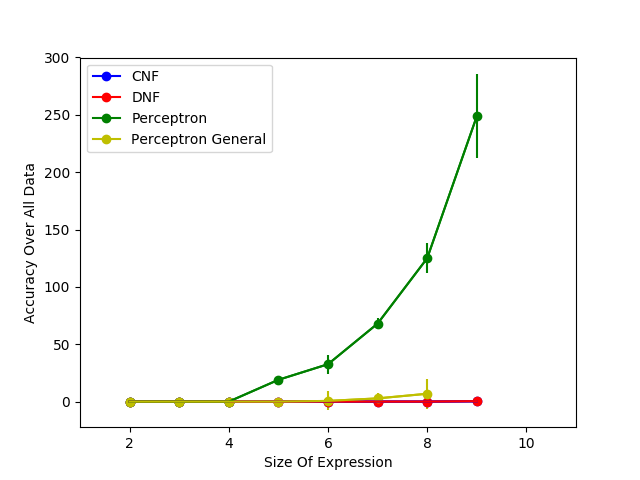
\includegraphics[width=\textwidth]{All-Peformance-Comparason.png}
    \caption{}
    \label{fig:peformance-comparason-all}
  \end{minipage}
  \begin{minipage}[b]{0.45\textwidth}
    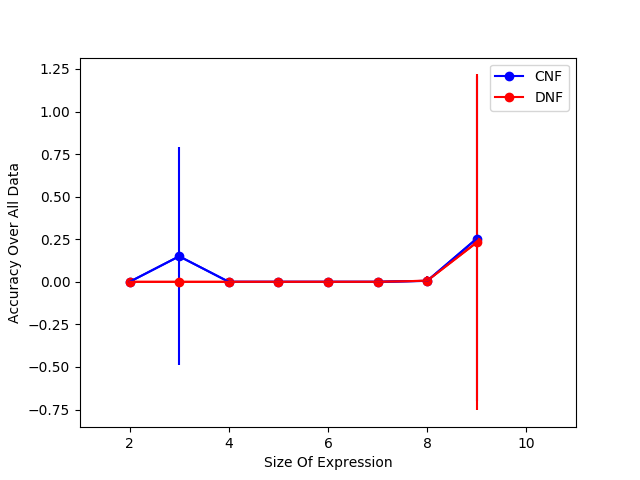
\includegraphics[width=\textwidth]{CNFvsDNF.png}
    \caption{}
    \label{fig:peformance-comparason-cnfdnf}
  \end{minipage}
  \hfill
\end{figure}

\section{LNF Network Generalization} \label{sec:lnfn-generalization}
These networks are able to perform as well as standard perceptron networks but so far they have been trained on a complete data set. In practice this will almost never be the case. Standard ANN's are widely used because of their ability to generalize. Here the generalization capability of LNFNs will be tested against that of MLPNs

\begin{figure}[H]
	\centering
	\begin{minipage}[t]{0.6\textwidth}
		\vspace{0px}
		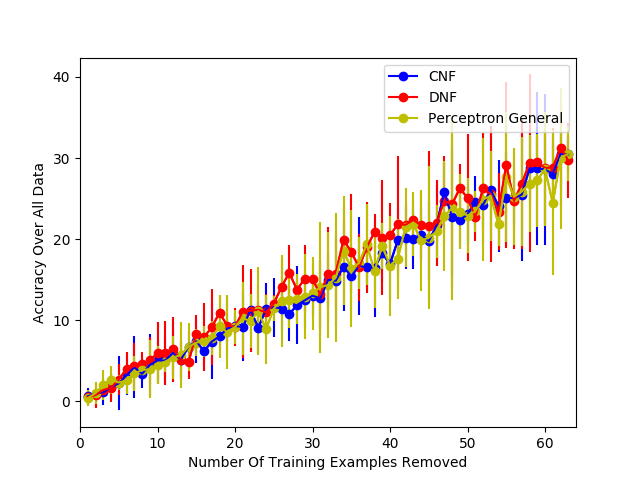
\includegraphics[width=\textwidth]{6-generalization.png}
		\caption{}
		\label{fig:generalization-peformance-6}
	\end{minipage}
	\begin{minipage}[t]{0.39\textwidth}
	\vspace{0px}
		Figure \ref{fig:generalization-peformance-6} shows a comparison between the generalization ability of CNF, DNF and Perceptron networks. The graph shows the performance over all training data when successively removing elements from the training set. It demonstrates that the CNF and DNF networks generalize as well as the perceptron networks when trained over boolean problems with 6 inputs, this trend continues as n increases up to 9. Training LNFNs on boolean problems with more than 9 inputs is to expensive.		
	\end{minipage}
	\hfill
\end{figure}

\section{LNF Network Rule Extraction} \label{sec:lnfn-rule-extraction}
Consider the weights for a logical neuron $W = \{w_1, ..., w_n\}$. These can be converted to $\epsilon_i = \sigma(w_i)$ where $\epsilon_i \in [0, 1]$ and represents the relevance input $x_i$ has on the neurons output.\\

To extract boolean rules from the network it must be possible to interpret each neuron as a logical function acting on a subset of its inputs. For this to be the case, at the conclusion of training either $\epsilon_i \approxeq 1$ or $\epsilon_i \approxeq 0$ needs to be true. If each $\epsilon_i$ is either 1 or 0 then the neuron is a logical function of the inputs which have corresponding $\epsilon \approxeq 0$.\\

Conjecture \ref{conj:lnfn-approach-binary} is the foundation of the following rule extraction algorithm, it was derived from experimental evidence by training LNFNs over complete truth tables and inspecting the weights. Ideally Conjecture \ref{conj:lnfn-approach-binary} would be proved, but that is out of scope for this report.

\begin{conjecture}
	For an LNFN network trained on a binary classification problem with boolean inputs as the loss approaches 0  (i.e. the correct CNF or DNF has been found) the weights $\{ w_1, ..., w_n \}$ approach $\infty$ or $-\infty$. Consequently each $\epsilon_i$ approaches 0 or 1.
	\label{conj:lnfn-approach-binary}
\end{conjecture}

The Algorithm displayed in figure \ref{alg:rule-extraction} extracts rules from CNFNs. It takes the output weights (ow) and hidden weights (hw) as input and outputs the a boolean expression. A similar algorithm can be derived for DNFNs, it is omitted but can be obtained by simply switching the logical operations around.

\begin{figure}[H]
	\begin{lstlisting}[mathescape=true]
atoms = $\{ x_1, \lnot x_1, ... x_n, \lnot x_n, \}$
	
function extractRulesCNFN(ow, hw)
  ow $= \sigma($ow$)$
  hw $= \sigma($hw$)$
  relvHidden = [hw[i] where ow[i] := 0]
		
  and = And([])
    for weights in relvHidden
      or = Or([atoms[i] where weights[i] := 0])
      and.add(or)
		
  return and
	\end{lstlisting}
	\caption{Rule Extraction Algorithm (for CNFN)}
	\label{alg:rule-extraction}
\end{figure}

In practice many clauses in the extracted expression contain redundant terms, such as clauses that are a tautology or a duplicate of another. Filtering these out is not an expensive operation.\\

Section \ref{sec:lnfn-generalization} discusses the generalization capabilities of LNFNs compared to MLPNs and shows that they are statistically equivalent. How does training over incomplete truth tables effect the generalization of extracted rules and what factors could influence this?\\

Consider $B$ to be the set of all boolean problems with $n$ inputs. What is the cardinality of $B$? There are $2^n$ rows in the truth table and $2^{2^n}$ ways to assign true/false values to these rows, each way corresponding to a different boolean function. Consequently $|B| = 2^{2^n}$. Consider some $b \in B$ represented by $2^n$ rows of a truth table, removing one row from the training data means there are now two possible functions that could be learnt, one where the removed row corresponds to true and the other to false. As more rows are removed this problem is compounded, if $m$ rows are taken then there are $2^m$ possible functions.\\

When constructing a CNF or DNF from a truth table (See Section \ref{subsec:construct-cnfdnf}) in the case of CNF only the rows corresponding to false are considered and for the DNF only rows corresponding to true. Despite the fact that if $m$ rows are removed from the training set then there are $2^m$ possible functions that could represent the partial truth table. Does this same principle apply to the rules extracted from CNF or DNF networks?

Figure \ref{fig:cnf-descrete-generalizatiion} shows how the rule set of an CNFN generalizes as examples are removed. Figure \ref{fig:dnf-descrete-generalizatiion} shows the same but for DNFNs.

\begin{figure}[H]
	\centering
	\begin{minipage}[b]{0.45\textwidth}
		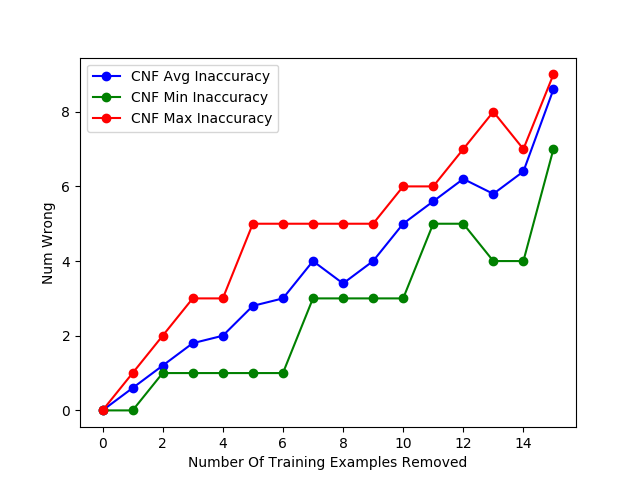
\includegraphics[width=\textwidth]{cnf-descrete-generalization.png}
		\caption{}
		\label{fig:cnf-descrete-generalizatiion}
	\end{minipage}
	\begin{minipage}[b]{0.45\textwidth}
		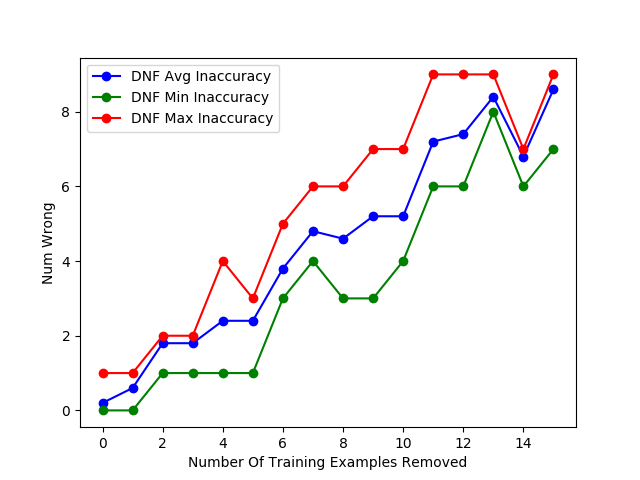
\includegraphics[width=\textwidth]{dnf-descrete-generalization.png}
		\caption{}
		\label{fig:dnf-descrete-generalizatiion}
	\end{minipage}
	\hfill
\end{figure}

In Figures \ref{fig:cnf-descrete-generalizatiion} \& \ref{fig:dnf-descrete-generalizatiion} the training examples which are removed get randomly selected. How is the performance effected if the removed examples are chosen more carefully? In the next experiment only examples corresponding to false are removed and the resultant training set is given to a DNFN.

\begin{figure}[H]
	\centering
	\begin{minipage}[b]{0.45\textwidth}
		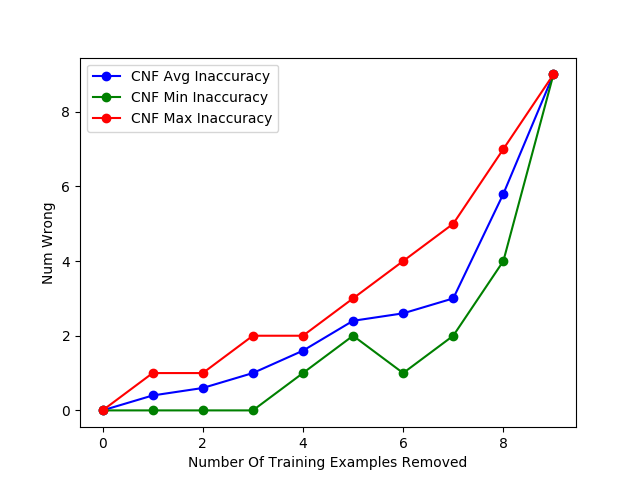
\includegraphics[width=\textwidth]{cnf-descrete-generalization-partial.png}
		\caption{}
		\label{fig:cnf-descrete-generalizatiion-partial}
	\end{minipage}
	\begin{minipage}[b]{0.45\textwidth}
		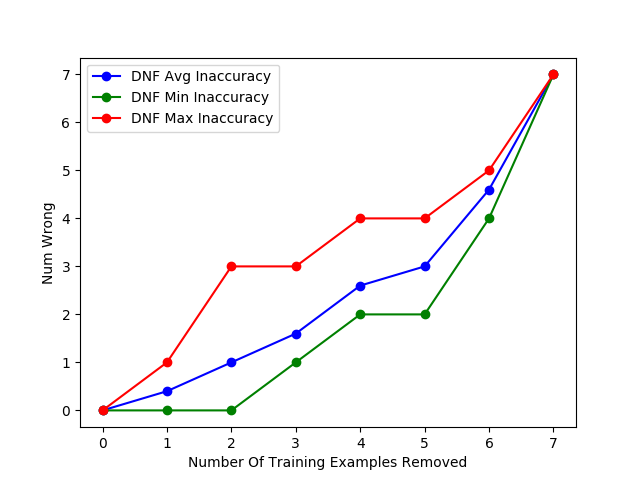
\includegraphics[width=\textwidth]{dnf-descrete-generalization-partial.png}
		\caption{}
		\label{fig:dnf-descrete-generalizatiion-partial}
	\end{minipage}
	\hfill
\end{figure}

Figures \ref{fig:cnf-descrete-generalizatiion-partial} \& \ref{fig:dnf-descrete-generalizatiion-partial} shown CNFNs and DNFNs trainined over partial data retrospectively. In the case of CNFNs only etries corosponding to true in the truth table are removed and for the DNFNs only false entries. These graphs show that careful removal of each training example does not result in rules that peform better.

\chapter{Expanding the Problem Domain of Logical Normal Form Networks} \label{C:investigation-of-lnfns}
The LNFNs presented in Chapter \ref{C:foundation-of-lnfns} have only been shown to be appiliciple when learning boolean truth tables. This chapter investigates extending LNFNs to support multi class classification problems and continous feature spaces.

\section{Multi-class Classification}
Extending an ANN to support multi class classification is achieved by adding more output neurons, one for each class. The value output neuron $i$ can be considered the probability of class $i$. The networks output is now a vector representing the class distribution. \\

For example if given a problem with 3 classes then $\{1,0,0\}$, $\{0,1,0\}$ and $\{0,0,1\}$ represent class 1, 2 and 3 retrospectively. The LNFN would have 3 output neurons, each representing a bit in the output vector. During the training process if the true class of an example was 1 then the desired output vector would be $\{1,0,0\}$.\\

This process of converting a categorical variable to a binary string is known as \textbf{One-Hot Encoding}

\begin{definition}
	An LNFN to solve a $k$ class classification problem is unchanged apart from the number of output neurons which is $k$.
\end{definition}

The Lenses problem \cite{Lichman:2013} is multi class and contains a natural rule system making it an ideal problem for evaluating LNFNs. Each example has four features, three are binary and one categorical (of size 3). Applying One-Hot encoding to the categorical variable yields a set of instances each with length 6.\\

The LNFN will be evaluated against an MLPN with a two layer structure where the layer width are $2 \cdot n$ and $n$ retrospectively.\\

The performance of the two classifiers will be compared using Leave-One-Out Cross-Validation. The structure of the MLPN differs in the number of hidden layers/units, there are two hidden layers, one with $2 \cdot n$ hidden units and the other with $n$

\begin{table}[H]
	\begin{center}
		\begin{tabular}{| c | c | c |}
			\hline
			& Error Rate & Error Rate CI (95\%) \\
			\hline
			\hline
			CNF Net & 0.0122 & (0.0000, 0.0417) \\
			\hline
			DNF Net & 0.0104 & (0.0000, 0.0417) \\
			\hline
			PCEP Net & 0.0000 & (0.0000, 0.0000) \\
			\hline
		\end{tabular}
	\end{center}
	\caption{Network Peformance On Lenses Problem}
	\label{tab:lenses-peformance-comp}
\end{table}

Table \ref{tab:lenses-peformance-comp} demonstrates that the CNF \& DNF Networks perform comparably to an MLPN as the confidence intervals for the errors overlap.\\ 

Now that the LNFN network has three output neurons it should be possible to extract three rules describing each of the classes. Consider that each problem instance is of the following form $\{a, b, c, d, e, f\}$ where $a,b,c,d,e,f$ are all atoms. $f$ refers to the \textit{tear production rate} being normal or reduced if $f = False$ or $True$ retrospectively. Giving a description of the other atoms is not beneficial as they refer to medical terms which are unimportant.\\

The following rules have been extracted from a CNFN after being trained over the complete Lenses data set. Any duplicate clause or Tautology has been filtered out, the resultant extracted formula has also been manually simplified (so they can be displayed and understood better).

\begin{itemize}
	\item \text{Class 1:} $(a \lor b \lor e) \land (a \lor \lnot d) \land (c \lor e) \land f$
	\item \text{Class 2:} $(a \lor b \lor \lnot c \lor d) \land \lnot e \land f$
	\item \text{Class 3:} $(\lnot a \lor b \lor c \lor \lnot f) \land (a \lor \lnot d \lor e \lor \lnot f) \land (\lnot b \lor c \lor d \lor \lnot f) \land (d \lor \lnot e \lor \lnot f)$
\end{itemize}

Immediately it is possible to find useful information about this problem that was not obvious before. For example $\lnot f = True \implies $ Class 3, or \textit{if the tear reduction rate is reduced then do not fit contact lenses}.



The DNFN might be more applicable as the rules will be more insightful. Each clause in the formulas represents a situation where the class is true. The formulae extracted from the DNFN confirm the previous knowledge extracted, $\lnot f = True \implies $ Class 3.

\begin{itemize}
	\item \text{Class 1:} $(a \land \lnot b \land \lnot c \land e \land f) \lor (\lnot a \land \lnot d \land e \land f)$
	\item \text{Class 2:} $(\lnot c \land \lnot e \land f) \lor (c \land d \land \lnot e \land f)$
	\item \text{Class 3:} $(\lnot a \land \lnot b \land c \land \lnot d) \lor (\lnot a \land d \land e) \lor \lnot f$
\end{itemize}

Table \ref{tab:lenses-rule-peformance-comp} demontres the peformance of extracted rules over the Lenses dataset. The confidence intervals of networks and rule sets overlap so there is no stistically significant difference between the network and rule set in terms of their accuracy on the data.

\begin{table}[H]
	\begin{center}
		\begin{tabular}{| c | c | c |}
			\hline
			& Rule Error Rate & Rule Error Rate CI (95\%) \\
			\hline
			\hline
			CNF Rules & 0.0122 & (0.0000, 0.0417) \\
			\hline
			DNF Rules & 0.0156 & (0.0000, 0.0417) \\
			\hline
		\end{tabular}
	\end{center}
	\caption{}
	\label{tab:lenses-rule-peformance-comp}
\end{table}

\section{Features with Continuous Domains}
The input features to an LNFN are probabilities, as such they are allowed to be continuous but must be in the range $[0, 1]$. Consider attempting to learn the Iris data set \cite{Lichman:2013} with an LNFN. One option would be to normalize all the variables to force them into the expected range $[0,1]$. The values of all the features after normalization are compatible with an LNFN, but consider the meaning, can these normalized features do not represent probabilities.\\

It is possible to think of these normalised features as the probability that the true value is the upper bound of the original range. For example if the features range from 0 to 2, and one example has a feature value of 1, when normalised it becomes $\frac{1}{2}$ or a 50\% probability of being a 2. For a moment forget about trying to find meaning in these normalised features. What happens if an LNFN is trained on the Iris problem? Table \ref{tab:iris-network-peformance-comp} gives the results of training the normalised Iris problem on LNF networks. The results show that while the peformance can very alot it is possible for both the CNF and DNF networks to obtain 100\% accuracy.

\begin{table}[H]
	\begin{center}
		\begin{tabular}{| c | c | c |}
			\hline
			& Error Rate & Error Rate CI (95\%) \\
			\hline
			\hline
			CNF Network & 0.027 & (0.000, 0.111) \\
			\hline
			DNF Network & 0.066 & (0.000, 0.156) \\
			\hline
		\end{tabular}
	\end{center}
	\caption{tab:iris-network-peformance-comp}
	\label{tab:iris-network-peformance-comp}
\end{table}

Given that the input features to the network are continous it is not possible to extract boolean rules. It is possible to find the most important features in each classification from inspecting the weights. If attempting to intepret these models meaning must be assigned to each of the normalised features. Consider an abatary (un-normalised) feature $f$. Assume $f \in [f_min, f_max]$ then the larger the normalised feature $f_N$ the closer its true value is to $f_max$. Similarly if $\lnot f_N = 1 - f_N$ is large then the true value is small.\\

The list below describes the attributes of each class on an CNF network which obtained an error rate of 0\% on the testing set. These discovered rules reveal intesting information about the dataset. Having a small petal width and length mean the class is more likely to be \textit{Iris Setosa}. Alternatively having a larget petal width means the instance is more likely to be \textit{Iris Virginica}.

\begin{figure}[H]
	\centering

	\begin{minipage}[p]{0.51\textwidth}
	 Finally the \textit{Iris Versicolour} rule is more complicated and seemes contridictory. If the instance has a small petal width and length but also has a large petal width or length.
\begin{enumerate}
	\item \textit{Iris Setosa: } Smaller \textbf{petal width} AND Smaller \textbf{petal length}
	\item \textit{Iris Versicolour: } Smaller \textbf{petal width} AND Smaller \textbf{petal length}. AND ( Larget \textbf{petal width} OR Larger \textbf{petal length} )
	\item \textit{Iris Virginica: } Larger \textbf{petal width}
\end{enumerate}
	\end{minipage}
	\hspace{4px}
	\begin{minipage}[p]{0.45\textwidth}
		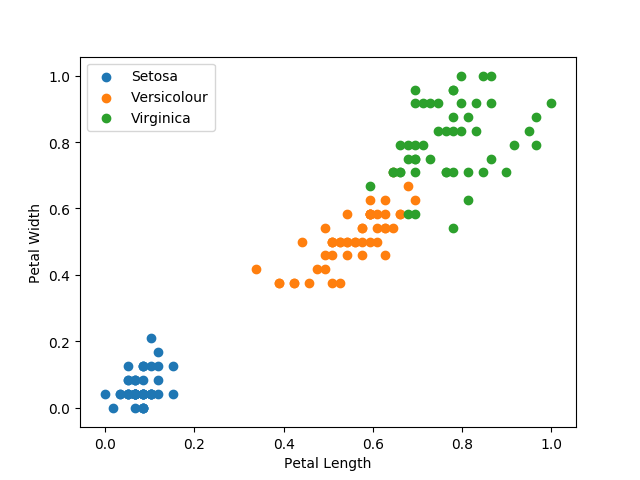
\includegraphics[width=\textwidth]{IrisData(petal(length-vs-width)).png}
		\caption{Scatter plot of Iris dataset, showing the petal length on the x-axis and petal width on the y-axis}
		\label{fig:iris-data-petal-length-vs-width}
	\end{minipage}
	\hfill
\end{figure}

Figure \ref{fig:iris-data-petal-length-vs-width} clearly demonstrats the rules for the two classes, \textit{Iris Setosa} and \textit{Iris Virginica}. The Figure also gives insite as to the meaning of the class rule for \textit{Iris Versicolour}, these instances are generally centered around the middle with a trend of increasing length and width. The two features \textbf{sepal width} and \textbf{sepal length} are used in the classification algorythm but have a very small weighting which is why they have been omitted.

\section{Discussion}
This chapter has demonstraited that LNFNs can be applied to more than just learning boolean truth tables. They have been shown to achieve good accuracy on multi class classification problems, with and without descrete input features.\\

In the context of the Lenses problem it was possible to extract boolean rules from the LNFNs which had a stistically equivelent peformance to the networks. These rules also provided insite into the problem which was not obvious from the data.\\

The LNFNs where able to achieve a low error rate (sometimes 0\%) on the Iris data set. It was possible to extract usful information from the trained models which highlighted the most important features when making classifications.

\chapter{Logical Neural Networks} \label{C:lnn}
This chapter discusses development of Logical Neural Networks as a generalization of LNFNs. There are two key issues with LNFNs. Firstly the number of hidden units becomes infeasible as the amount of inputs increases. Secondly if the problem size is small enough and the network can be trained the volume of hidden neurons allows for the possibility to memorise the input data.\\

Using what has been learnt about LNFNs the class of Logical Neural Networks (LNNs) can be defined.

\begin{definition}
	A \text{Logical Neural Network} is an ANN where each neuron has a noisy activation.
\end{definition}

LNNs have a more flexible structure, allowing for deeper networks and hidden layers with a variable number of neurons. The current LNN model has been shown to have poor performance when compared to a Multi-Layer Perceptron Network \cite{LearningLogicalActivations}. An LNN, consisting of Noisy-OR hidden units and Noisy-AND outputs, was shown to perform worse than an MLPN. 

There are two key issues caused by removing the restrictions imposed by the LNFN definition (Definition \ref{def:lnfn}) which must be addressed 

\begin{enumerate}
	\item Noisy neurons do not have the capacity to consider the presence of the negation of an input. This was a problem for LNFNs as well, however given that only the negations of atoms need to be considered to learn a CNF or DNF it was easily fixed by presenting the network with each atom and its negation. The problem can not be solved so easily for LNNs. A boolean formula can not always be represented by only AND and OR gate, i.e the set of operations $\{AND, OR\}$ is not functionally complete. 
	
	\item Another problem faced by LLNs that are not restricted to be ether a CNFN or DNFN is that the structure of the network will have a higher impact on whether the problem can be learnt. 
\end{enumerate}

Resolving Issue 1 involves making our operation set functionally complete, this requires the $NOT$ operation. There are two ways to include the $NOT$ operation in the LNNs, one is to simply augment the inputs to each layer appending so it receives the input and its negation. Another is to derive a parametrisation of Noisy gates which can learn to negate inputs. However both these have no way to enforce mutual exclusivity between an input and its negation.\\

\section{Modified Logical Neural Network} \label{sec:modified-lnn}
\subsection{Connections Between Layers \& Parameters}
Figure \ref{fig:modified-lnn-structure} provides a new structure for the connections between the lectures.

\begin{figure}[H]
	\centering
	\begin{minipage}[b]{0.9\textwidth}
		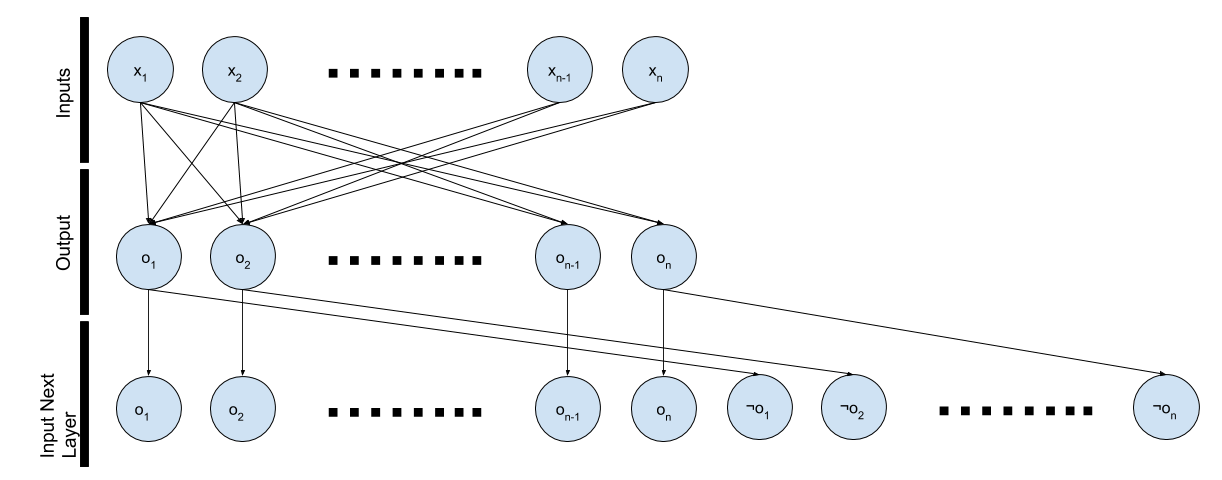
\includegraphics[width=\textwidth]{Modified-LNN-Structure.png}
		\caption{}
		\label{fig:modified-lnn-structure}
	\end{minipage}
	\hfill
\end{figure}


Figure \ref{fig:modified-lnn-structure} shows the new LNN structure which includes an implicit NOT operation. The input to each layer consists of the true output of the previous plus the negated output from the last layer. If a layer has 20 outputs then there are 40 inputs to the following layer.\\

\subsection{Softmax Output Layer}
The softmax function takes a vector of real values to a vector of values in the range $[0,1]$ that equal 1 when summed. The softmax function highlights the difference between the maximum and smaller values by increasing this difference. It is used in multiclass classification to generate a probability distrubution over the different outcomes and promote mutual exclusivity between the different classes.\\

The old LNN structure does not include a Softmax layer as the output layer. A traditional Softmax layer would not be effective as the neuron outputs are limited to the range $[0,1]$. Figure \ref{fig:softmax-failure} shows an example of the softmax function on probabilities, insted of highilight the difference between 0.1 and 0.9 the resulting vector has the values closer together.

\begin{figure}[H]
\begin{align*}
A &= \{01, 0.9\}\\
SoftMax(A) &= \{ \frac{e^{0.1}}{e^{0.1} + e^{0.9}}, \frac{e^{0.9}}{e^{0.1} + e^{0.9}} \}\\
&\approxeq \{ 0.29, 0.71 \}
\end{align*}
\caption{Demonstration of Softmax on probabilities}
\label{fig:softmax-failure}
\end{figure}

Consider the following vector of probabilities $P = \{p_1, ..., p_n\}$ where $p_i$ is the probability the given example belongs to class $i$. Then define $p_i^{'} = \frac{p_i}{\sum_j p_j}$, performing this action to generate a vector $P^{'}$ where each of the classes are mutually exclusive. This operation can be thought of as a "Logical Softmax".\\

Adding a "Logical Softmax" may guarantee mutual exclusivity of each classes but will it cause the network to be less interpretable? Consider that without with no softmax then the network outputs directly represent the probabilities that the input vector is class $k$ given the parameters. Once the "Logical Softmax" has been introduced then it becomes less clear what the non softmaxed probabilities represent. The softmax introduces a dependency between the output neurons of the network which might cause a decrease in intepretability. This is a question which will be explored during experimentation with the modified LNN architecture.




\chapter{Evaluation Of Logical Neural Networks} \label{C:evaluation-lnn}
To evaluate Logical Neural Networks their performance and intepretability are explored. In Chapter \ref{C:backgroundsurvey} different methods for evaluating the intepretability of models where presented. The method used in this report is \textit{"Application-Grounded Evaluation"} \cite{doshi2017towards} which relies on domain experts to assess the intepretability of a model. The two problems MNIST \cite{mnistlecun} and Tic-Tac-Toe \cite{Lichman:2013} will be used in this evaluation.\\

These problems are a sutable choice as their simplisity makes most humans domain experts. Tic-Tac-Toe has a simple rule set that is easy to comprehend. MNIST is the problem of classifying handwritten digits, a task that is peformed on a daily bais by most humans.\\

There are \textbf{5} criteria that will be used for this evaluation.

\begin{enumerate}
	\item Performance comparison between the old and new Logical Neural Network Structures.
	\item Performance comparison between Multi Layer Perceptron Network and Logical Neural Networks.
	\item Performance comparison between Logical Neural Networks with and without a Logical Softmax.
	\item Comparison of intepretability between MLPNs and new/old LNNs
	\item Comparison of intepretability between MLPNs (using LIME) and new/old LNNs
\end{enumerate}

It was conjectured that AND neurons where not effective for low level feature extraction \cite{LearningLogicalActivations}. Throughout this evaluation, AND neurons will be used in the first hidden layer to determine whether this conjecture holds.


\section{Performance of Logical Neural Networks} \label{sec:lnn-eval-peformance}
To evaluate the performance of Logical Neural Networks (LNNs) a number of different configurations will be trained on the MNIST dataset. Each experement will be trained for 30 epochs. Any experements with an LNN archetchure will be trained with and without an Logical Softmax

\begin{enumerate}
	\item \textbf{(OR $\rightarrow$ AND) Old Architecture:} This will consist of 30 hidden OR neurons. \label{lnn-eval-arch-1}
	\item \textbf{(OR $\rightarrow$ AND) Architecture:} Same as \ref{lnn-eval-arch-1} but with the new LNN architecture \label{lnn-eval-arch-2}
	\item \textbf{(AND $\rightarrow$ OR) Architecture:} 30 hidden AND neurons \label{lnn-eval-arch-3}
	\item \textbf{(OR $\rightarrow$ AND $\rightarrow$ AND) Architecture: } 60 hidden OR neurons, 30 hidden AND neurons\label{lnn-eval-arch-4}
	\item \textbf{(OR) Architecture:} \label{lnn-eval-arch-5}
	\item \textbf{(AND) Architecture:} \label{lnn-eval-arch-6}
	\item \textbf{(AND) Old Architecture:} \label{lnn-eval-arch-7}
\end{enumerate}

\paragraph{Results}
Each network is trained 30 times to average the results over different initial conditions. Tables \ref{tab:mnist-sigmoid-peformance-results} \& \ref{tab:mnist-lnn-peformance-results} display the Sigmoid and LNN results retrespectively. Each error rate reported is obtained from an unseen test set.

\begin{table}[H]
	\begin{center}
		\begin{tabular}{| c | c | c | c | c |}
			\hline
			\textbf{Network Config} & \textbf{Error Rate} & \textbf{Error Rate CI} & \textbf{Error Rate (with SM)} & \textbf{Error Rate CI (with SM)}\\
			\hline
			\hline
			\textbf{60 $\rightarrow$ 30} & 0.034 & (0.031, 0.038) & 0.035 & (0.030, 0.040)\\
			\textbf{30} & 0.046 & (0.042, 0.050) & 0.045 & (0.041, 0.050)\\
			\textbf{N/A} & 0.085 & (0.085, 0.085) & 0.084 & (0.084, 0.084)\\
			\hline
		\end{tabular}
	\end{center}
	\caption{Results of experiments with Sigmoid models}
	\label{tab:mnist-sigmoid-peformance-results}
\end{table}

\begin{table}[H]
	\begin{center}
		\begin{tabular}{| c | c | c | c | c |}
			\hline
			\textbf{Network Config} & \textbf{Error Rate} & \textbf{Error Rate CI} & \textbf{Error Rate (LSM)} & \textbf{Error Rate CI (LSM)}\\
			\hline
			\hline
			\textbf{(OR $\rightarrow$ AND) Old } & 0.105 & (0.098, 0.115) & 0.048 & (0.043, 0.052)\\
			\textbf{(OR $\rightarrow$ AND) } & 0.088 & (0.079, 0.094) & 0.042 & (0.039, 0.046)\\
			\textbf{(AND $\rightarrow$ OR) } & 0.098 & (0.073, 0.141) & ? & ?\\
			\textbf{(OR $\rightarrow$ AND $\rightarrow$ AND) } & 0.053 & (0.046, 0.060) & 0.032 & (0.029, 0.036)\\
			\textbf{(OR) } & 0.382 & (0.381, 0.384) & 0.334 & (0.331, 0.336)\\
			\textbf{(AND) } & 0.137 & (0.135, 0.139) & 0.076 & (0.075, 0.079)\\
			\textbf{(AND) Old} & 0.312 & (0.311, 0.314) & 0.111 & (0.109, 0.114)\\
			\hline
		\end{tabular}
	\end{center}
	\caption{Results of experiments with Logical Neural Network models}
	\label{tab:mnist-lnn-peformance-results}
\end{table}

The experemental results lead to the folowing conclusions
\begin{enumerate}
	\item \textit{New LNN Architecture Gives Better Performance Than the Old:} The confidence intervals for test set performance do not overlap for Archetcures \textbf{(OR $\rightarrow$ AND) Old} and \textbf{(OR $\rightarrow$ AND)} (without LSM). This can also be observed from Archetchures \textbf{(AND) Old} and \textbf{AND}.
	
	\item \textit{Adding An LSM Improves Performance:} Every LNN using the new architecture gets a statistically significant performance increase when a LSM is added.

	\item \textit{It Is Unclear What Provides The Largest Improvement, New Strucure or LSM:} The experements show that both the new archetchure and LSM give a stistically significant improvement in peformance. From observing \textbf{(OR $\rightarrow$ AND) Old} and \textbf{(OR $\rightarrow$ AND)} (with LSM) it is possible to see that when a LSM is added then the change in archetchure does not introduce an increase in peformance. However the oposite is true when comparing the (AND) and (AND) Old networks.
\end{enumerate}

\section{Intepretability of Logical Neural Networks}
There are two cases of intepretability. In the situation where input and outputs are descrete then intepretablity becomes Rule Extraction. The other situation is where the inputs are continous.

\subsection{Discrete Case (Rule Extraction)}
To assess the rule extraction of LNNs the Tic Tac Toe  \cite{Lichman:2013} problem will be the becnchmark. 


\begin{figure}[H]
	\centering
	\begin{minipage}[t]{0.5\textwidth}
		\vspace{0px}
		This problem involves classifying tic-tac-toe endgame boards and determining whether 'x' can win . There are 9 categorical attributes, representing each cell of the board, each attribute can be 'x' (x has a piece here), 'o' ( o has a piece here) or 'b' (blank).\\
	
		This gives a total of 27 attributes after converson to a binary string. There are a total of 958 instances, 70\% of which will be used for training, the rest for testing.  Using the new LNN with the structure described in Figure \ref{fig:tic-tac-toe-net} (using 30 hidden OR neurons) is able to achieve an error rates displayed in Table \ref{tab:tic-tac-toe-lnn-peformance-results}. Each experiment is averaged over 30 runs
	\end{minipage}
	\hspace{1px}
	\begin{minipage}[t]{0.48\textwidth}
		\vspace{0px}
		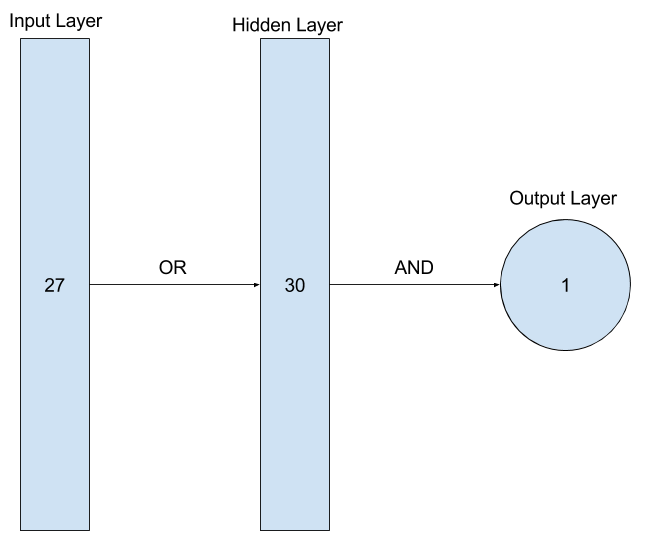
\includegraphics[width=\textwidth]{Tic-Tac-Toe-Net.png}
		\caption{Network archetchure for learning Tic-Tac-Toe}
		\label{fig:tic-tac-toe-net}
	\end{minipage}
	\hfill
\end{figure}



\begin{table}[H]
	\begin{center}
		\begin{tabular}{| c | c | c | c | c |}
			\hline
			\textbf{} & \textbf{Net Error Rate} & \textbf{Net Error Rate CI} & \textbf{Rule Error Rate} & \textbf{Rule Error Rate CI 95\%}\\
			\hline
			\hline
			\textbf{Training} & 0.0035 & (0.0035, 0.0035) & 0.0000 & (0.0000, 0.0000)\\
			\textbf{Testing} & 0.0015 & (0.0015, 0.0015) & 0.0259 & (0.0104, 0.0451)\\
			\hline
		\end{tabular}
	\end{center}
	\caption{Results of experiments with Logical Neural Networks on the Tic Tac Toe problem}
	\label{tab:tic-tac-toe-lnn-peformance-results}
\end{table}

If insted ANDs are used as the hidden nerons and ORs for the outputs then the LNN is able to achieve stistically equivelent peformance to the archetchure in Figure \ref{fig:tic-tac-toe-net}. Table \ref{tab:tic-tac-toe-lnn-peformance-results-and-or} shows the results from these experements.

\begin{table}[H]
	\begin{center}
		\begin{tabular}{| c | c | c | c | c |}
			\hline
			\textbf{} & \textbf{Net Error Rate} & \textbf{Net Error Rate CI} & \textbf{Rule Error Rate} & \textbf{Rule Error Rate CI 95\%}\\
			\hline
			\hline
			\textbf{Training} & 0.0035 & (0.0035, 0.0035) & 0.0000 & (0.0000, 0.0000)\\
			\textbf{Testing} & 0.0015 & (0.0015, 0.0015) & 0.0038 & (0.0, 0.0139)\\
			\hline
		\end{tabular}
	\end{center}
	\caption{Results of experiments with Logical Neural Networks on the Tic Tac Toe problem on a AND - OR Network}
	\label{tab:tic-tac-toe-lnn-peformance-results-and-or}
\end{table}

These experiments provide strong evidence against the conjecture stating that ANDs are not effective for extracting low level features.

\subsubsection{Evaluation of LNN Rules}
Figure \ref{fig:tic-tac-toe-rule-example} shows a rule taken at random from the AND OR network. This rule is saying that if the middle column contains all X's then X has won. There is redundancy in these rules as a cell can only be occupied by either an X, O or nothing.

\begin{figure}[H]
	\centering
	\begin{minipage}[t]{0.3\textwidth}
		\vspace{0px}
		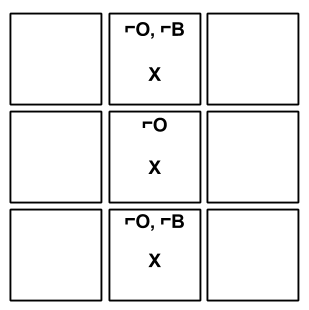
\includegraphics[width=\textwidth]{TicTacToe-RuleExample.png}
		\caption{A pictorial example of a rule extracted from the AND OR network}
		\label{fig:tic-tac-toe-rule-example}
	\end{minipage}
	\hspace{1cm}
	\begin{minipage}[t]{0.6\textwidth}
		\vspace{0px}
		A future goal might be to implement a way to build in mutual exclusivity of attributes into the network, this could result in further simplification of rules.\\

		The rule extraction algorithm given in Figure \ref{alg:rule-extraction} is an electic algorithm as this category describes algorithms that examine the network at the neuron level but extract rules which represent the network as a whole \cite{tickle1998truth}. The algorithm is not portable as it can only be applied to networks with the LNN architecture.\\

	Finally what is the quality of the rules extracted from LNN, this is measured by the Accuracy, Fedelity, Consistency and Comprehensibility \cite{andrews1995survey}.
	\end{minipage}
	\hfill
\end{figure}

\begin{enumerate}
	\item \textbf{Accurate:} As demonstrated experimentally the extracted rules are able to generalise well to unseen examples.
	\item \textbf{Fedelity:} The experiments show that the rules perform very similar to the network they where extracted from as both have a similar performance on the testing set.
	\item \textbf{Consistency:} These rule sets are consistent, shown by the low error rate when the neural network is trained from a number of different initial conditions.
	\item \textbf{Comprehensibility:} The upper limit of the size of the rules is related to the number of layers and neurons. The OR AND model obtains a complex set of rules, with a total 35 of the clauses. The AND OR model only utilizes 11 clauses. The structure also contributes to the comprehensibility of the rules. For instance each clause in the AND OR rules represent a situation where the rule set is true. Where as in the OR AND model each clause must true.
\end{enumerate}

\subsection{Continuous Case}
In the continuous case extracting boolean rules is not possible as each input no longer represents a boolean but rather a degree of truth. In terms of MNIST, being able to construct an image representing how relevant each input feature is to each of the possible output neurons would allow visual verification that the network has learnt something meaninful.\\

The weights from one layer to another directly correspond to how much influence the corresponding input has. Consquently determining the influence that the inputs to a layer have on the outputs of the layer is not a diffcult task. For example trying to compute the influence each $x_i$ has on the output of some $h_j$. However computing the influence that a neuron has across layers is not so simple. This is the case of asking how $x_i$ influences the output of $o_j$.

\begin{figure}[H]
	\centering
	\begin{minipage}[t]{0.5\textwidth}
		\vspace{0px}
		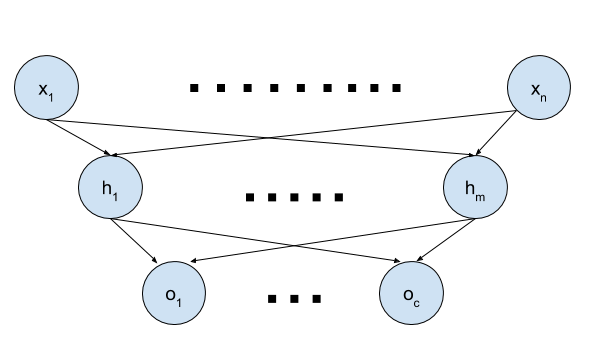
\includegraphics[width=\textwidth]{NetworkExample.png}
		\caption{Example Network}
		\label{fig:network-example}
	\end{minipage}
	\hspace{1px}
	\begin{minipage}[t]{0.45\textwidth}
		\vspace{2px}
	Consider this problem of trying to determine how each $x_i$ effects each $o_j$ and why it might be diffcult. In essence it equivalent to trying to find $\epsilon^{'}_i$ in Equation \ref{equ:interpetation-across-layers}. Note that exponent on each $\epsilon$ refers to the neuron it belongs to.

		\begin{align}
			(\epsilon^{'}_i)^{x_i} = \prod_{k = 0}^{m} (\epsilon^{o_j}_m)^{\prod_{b = 0}^{n} (\epsilon^{h_k}_b)^{x_b}}
			\label{equ:interpetation-across-layers}
		\end{align}
	\end{minipage}
	\hfill
\end{figure}

This new $\epsilon$ is dependent on all the other $x_i$'s, not just the one of interest. Consequently it is only possible to directly compute the influence of the input features with respect to the output from first layer of hidden neurons. Intepreting Multi Layer LNNs insted will be achieved by displaying the most relevent hidden features for a specific classification. Intepretability will be assessed by comparing various MNIST models using the new architecture again each other but also the original LNN model. Part of this assessment will be to determine what effects the LSM has on the model interpretation.

\subsubsection{No Hidden Layer Networks}


\paragraph{Sigmoid Network}
In the depictions of weights from a sigmoid network the blue represents a negative value and the red represents are positive weights. The features do not appear to represent any intepretable features of the digits.

\begin{figure}[H]
	\captionsetup{labelformat=empty}
	\centering
	\begin{minipage}[b]{0.19\textwidth}
		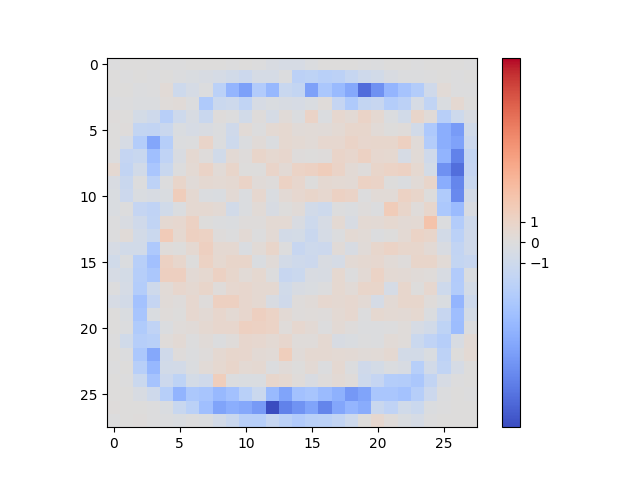
\includegraphics[width=\textwidth]{Sigmoid(NO-Hidden)/Layer0-Neuron-0.png}
		\caption{Digit 0}
	\end{minipage}
	\begin{minipage}[b]{0.19\textwidth}
		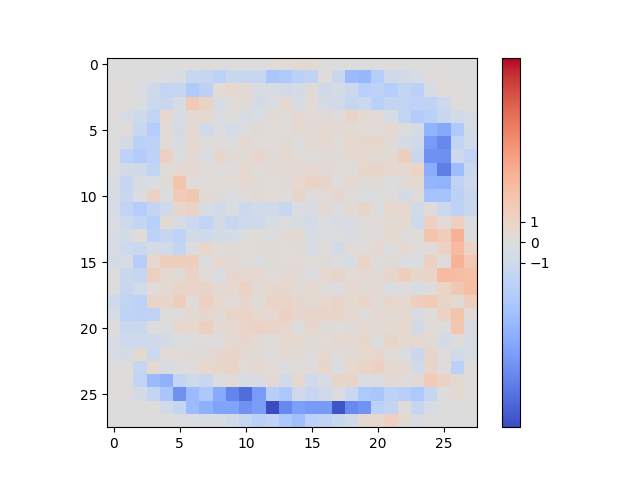
\includegraphics[width=\textwidth]{Sigmoid(NO-Hidden)/Layer0-Neuron-2.png}
		\caption{Digit 2}
	\end{minipage}
	\begin{minipage}[b]{0.19\textwidth}
		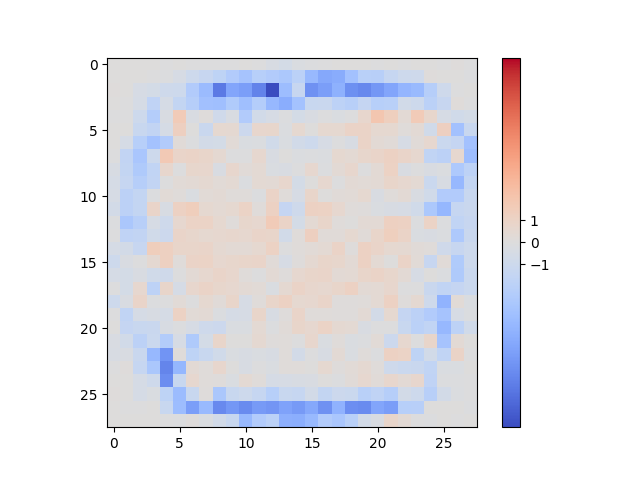
\includegraphics[width=\textwidth]{Sigmoid(NO-Hidden)/Layer0-Neuron-4.png}
		\caption{Digit 4}
	\end{minipage}
	\begin{minipage}[b]{0.19\textwidth}
		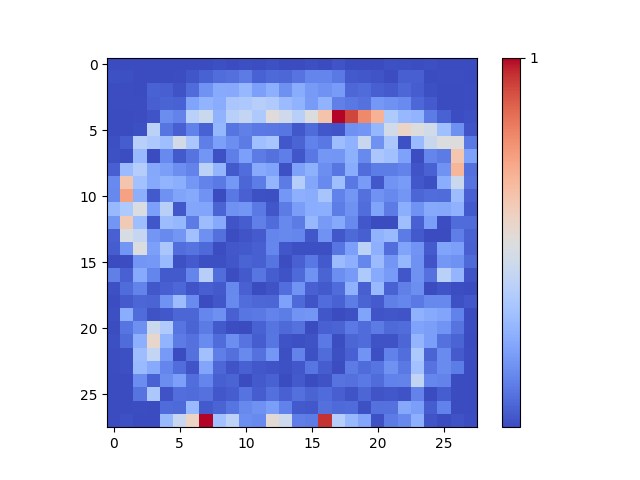
\includegraphics[width=\textwidth]{Sigmoid(NO-Hidden)/Layer0-Neuron-7.png}
		\caption{Digit 7}
	\end{minipage}
	\begin{minipage}[b]{0.19\textwidth}
		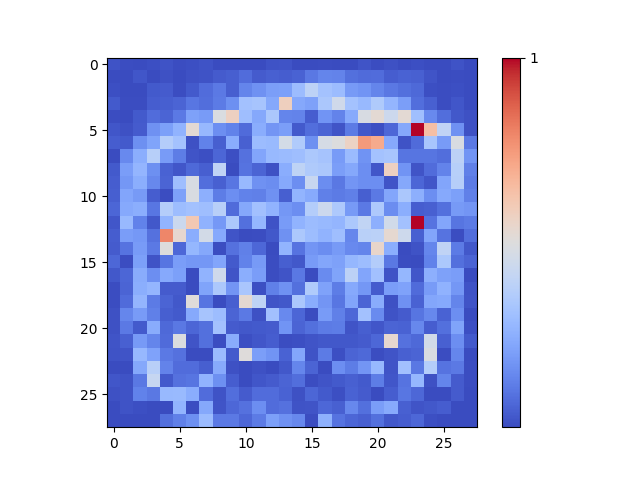
\includegraphics[width=\textwidth]{Sigmoid(NO-Hidden)/Layer0-Neuron-9.png}
		\caption{Digit 9}
	\end{minipage}
	\hfill
	\caption{Figures representing the output neurons of a sigmoid neural network with no hidden layers}
\end{figure}


\paragraph{AND Network Old Architecture (With and With Out LSM)}
The images in Figure \ref{fig:and-net-old-archetchure-interp} represent how relvent each input feature is towards a possitive classification of the digits 0, 2, 4, 7 and 9. The top and bottom rows represents the relevences for an AND archetchure with and without LSM retrespectively. The darker pixles represent more relevent features, where white is completly irrelevent.\\

The network without an LSM is using the pixels which occur in all representations of each digit. Whereas the network with an LSM is using the average border to achieve its classifications. Both models are intepretable as it is possible to understand the logic used in their decision making. Each of the models describe the probelm in a different way, uncovering different information. The model without an LSM shows describes what is common between every drawing of that digit. The model with an LSM describes which parts of each digit vary the most/least. The benefit of the model with an LSM is that the pictorial representations appear to look more like the the digits which they classify. However the model without an LSM has a sparser representation so the model is depnedent on less information.

\begin{figure}[H]
	%\captionsetup{labelformat=empty}
	\centering
	\begin{minipage}[b]{0.19\textwidth}
		\captionsetup{labelformat=empty}
		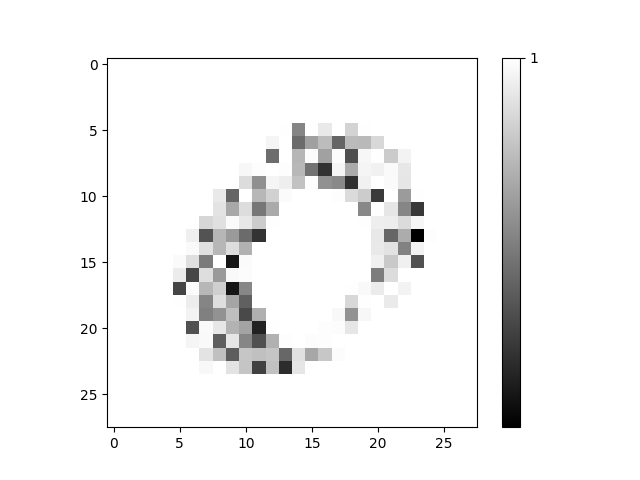
\includegraphics[width=\textwidth]{AND-OLD(LSM)/Layer0-Neuron-0.png}
		\caption{Digit 0}
	\end{minipage}
	\begin{minipage}[b]{0.19\textwidth}
		\captionsetup{labelformat=empty}
		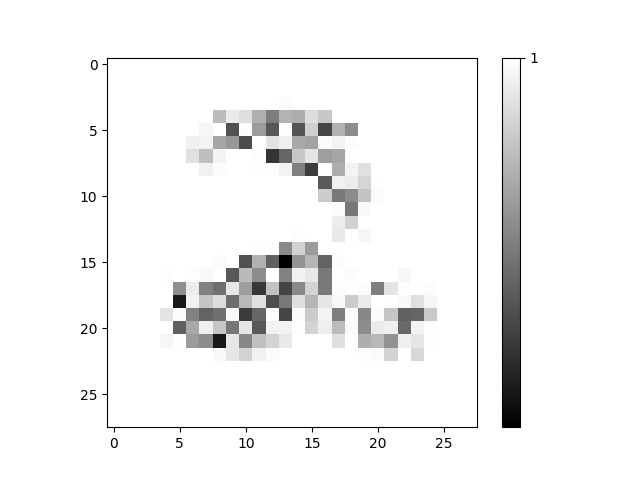
\includegraphics[width=\textwidth]{AND-OLD(LSM)/Layer0-Neuron-2.png}
		\caption{Digit 2}
	\end{minipage}
	\begin{minipage}[b]{0.19\textwidth}
		\captionsetup{labelformat=empty}
		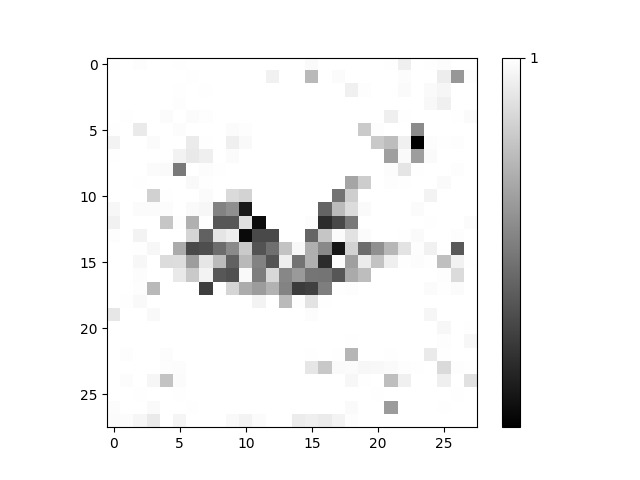
\includegraphics[width=\textwidth]{AND-OLD(LSM)/Layer0-Neuron-4.png}
		\caption{Digit 4}
	\end{minipage}
	\begin{minipage}[b]{0.19\textwidth}
		\captionsetup{labelformat=empty}
		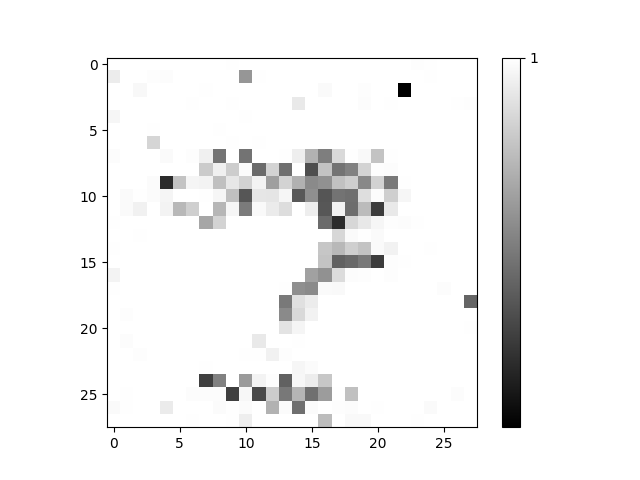
\includegraphics[width=\textwidth]{AND-OLD(LSM)/Layer0-Neuron-7.png}
		\caption{Digit 7}
	\end{minipage}
	\begin{minipage}[b]{0.19\textwidth}
		\captionsetup{labelformat=empty}
		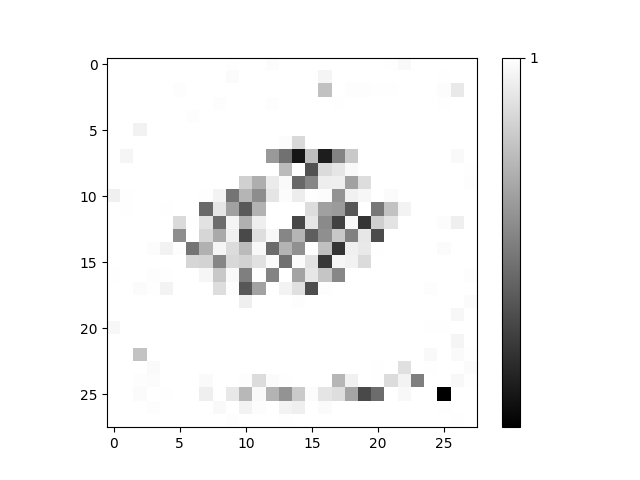
\includegraphics[width=\textwidth]{AND-OLD(LSM)/Layer0-Neuron-9.png}
		\caption{Digit 9}
	\end{minipage}
	\hfill
	\begin{minipage}[b]{0.19\textwidth}
		\captionsetup{labelformat=empty}
		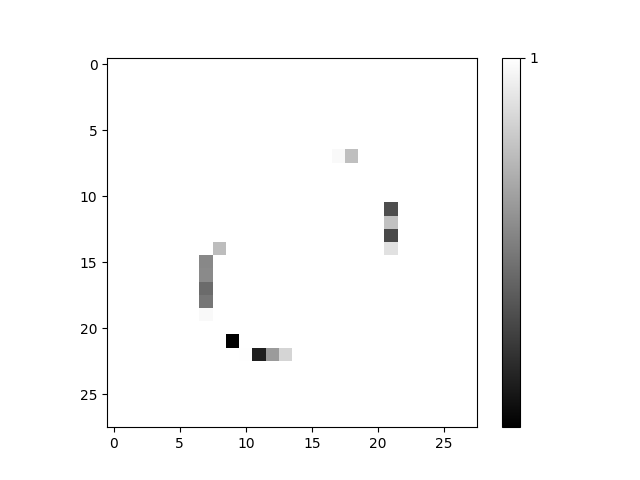
\includegraphics[width=\textwidth]{AND-OLD(NO-LSM)/Layer0-Neuron-0.png}
		\caption{Digit 0}
	\end{minipage}
	\begin{minipage}[b]{0.19\textwidth}
		\captionsetup{labelformat=empty}
		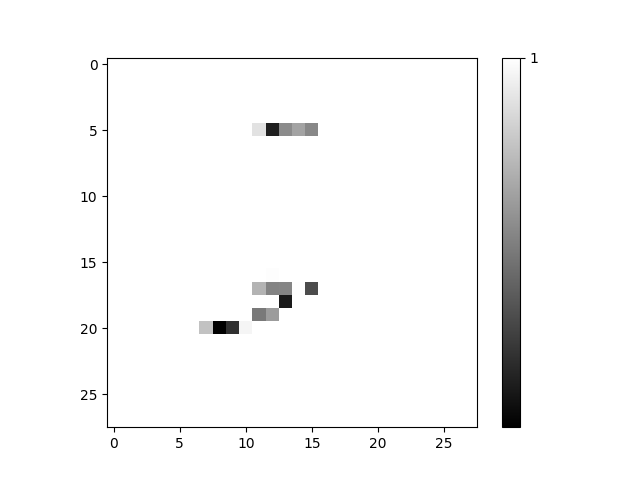
\includegraphics[width=\textwidth]{AND-OLD(NO-LSM)/Layer0-Neuron-2.png}
		\caption{Digit 2}
	\end{minipage}
	\begin{minipage}[b]{0.19\textwidth}
		\captionsetup{labelformat=empty}
		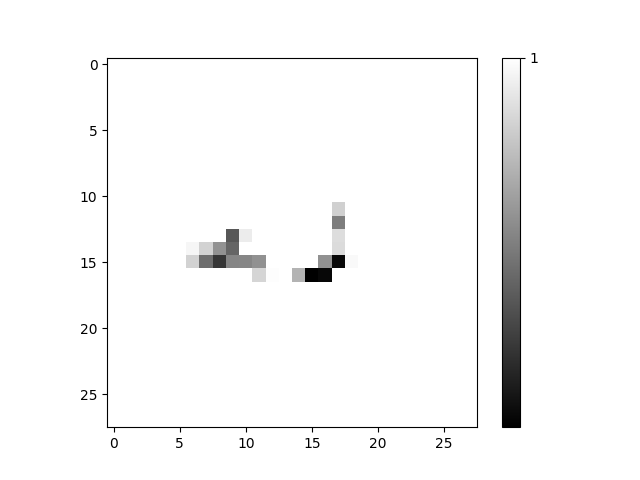
\includegraphics[width=\textwidth]{AND-OLD(NO-LSM)/Layer0-Neuron-4.png}
		\caption{Digit 4}
	\end{minipage}
	\begin{minipage}[b]{0.19\textwidth}
		\captionsetup{labelformat=empty}
		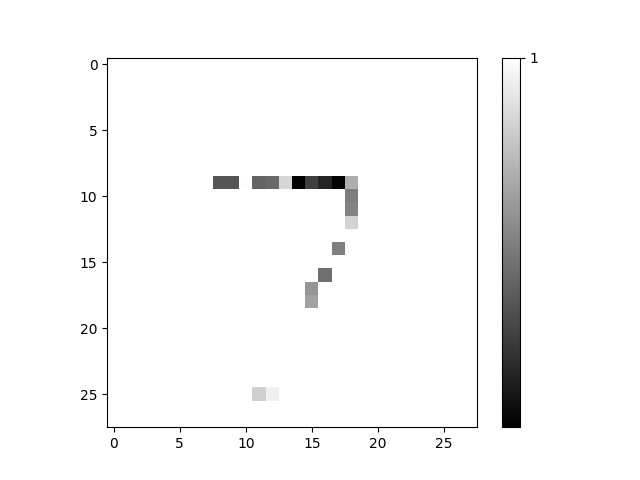
\includegraphics[width=\textwidth]{AND-OLD(NO-LSM)/Layer0-Neuron-7.png}
		\caption{Digit 7}
	\end{minipage}
	\begin{minipage}[b]{0.19\textwidth}
		\captionsetup{labelformat=empty}
		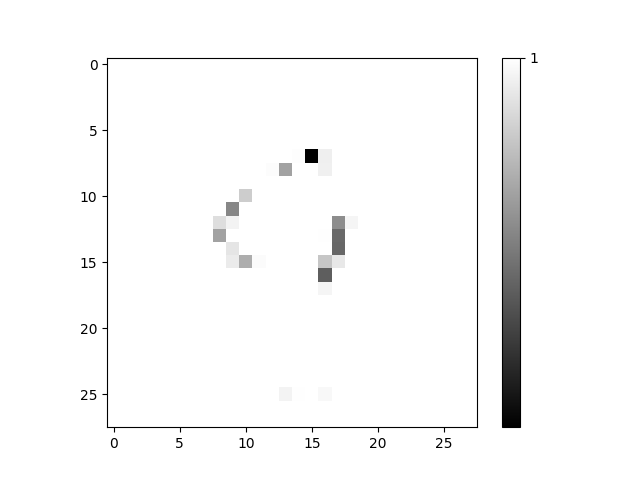
\includegraphics[width=\textwidth]{AND-OLD(NO-LSM)/Layer0-Neuron-9.png}
		\caption{Digit 9}
	\end{minipage}
	\hfill
	\caption{Figures representing the weighted connections between the inputs and outputs in an AND network with the old archetchure. Top row is with an LSM and bottom row is with out an LSM}
	\label{fig:and-net-old-archetchure-interp}
\end{figure}

\paragraph{AND Network (With LSM)}
The model here is an AND network running on the new archtchure (which considers the NOTs of inputs) with an LSM. The new archetchure means that each input feature can positively contribute to a classification or negatively contribute (i.e. if its present then the classification is less likely). Figure \ref{fig:and-net-new-archetchure-with-lsm-interp} shows the how relevent each input feature is with regards to a positive or negative classification for the digits 0, 2, 4, 7 and 9. The top row of images represent positively weighted inputs and the bottom row represents the negatively weighted inputs.\\

The inputs which are positively weighted are the pixels that occur in many of the representations of the digit. Negatively weighted inputs represent the border of the digit, if pixels on this border are present then the neuron is less likely to be active. Using the classification of 0 as an example, the network does not like pixels in the middle as the centre of a zero should be empty. The outer circle represents the border of the average 0, if these pixels are present then its less likely to be a zero as most instances of a 0 do not have pixels present there.

\begin{figure}[H]
	%\captionsetup{labelformat=empty}
	\centering
	\begin{minipage}[b]{0.19\textwidth}
		\captionsetup{labelformat=empty}
		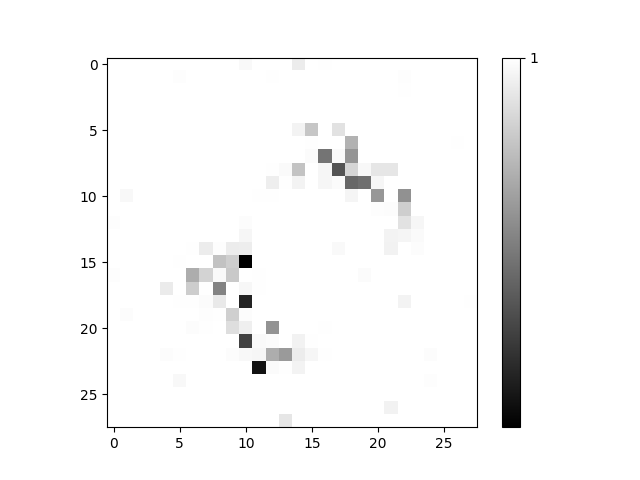
\includegraphics[width=\textwidth]{AND(LSM)/Positive/Layer0-Neuron-0.png}
		\caption{Digit 0}
	\end{minipage}
	\begin{minipage}[b]{0.19\textwidth}
		\captionsetup{labelformat=empty}
		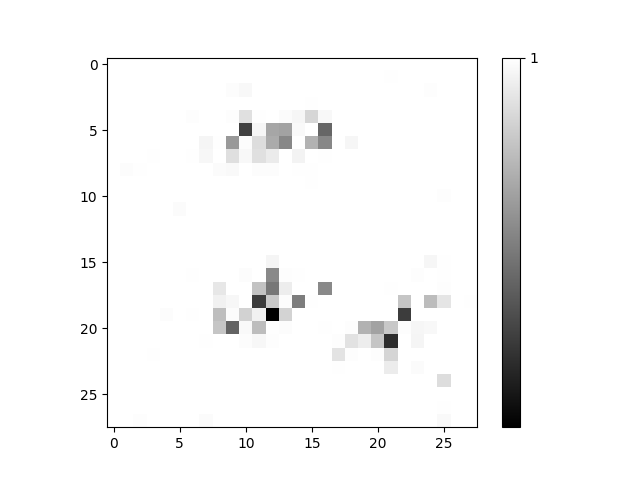
\includegraphics[width=\textwidth]{AND(LSM)/Positive/Layer0-Neuron-2.png}
		\caption{Digit 2}
	\end{minipage}
	\begin{minipage}[b]{0.19\textwidth}
		\captionsetup{labelformat=empty}
		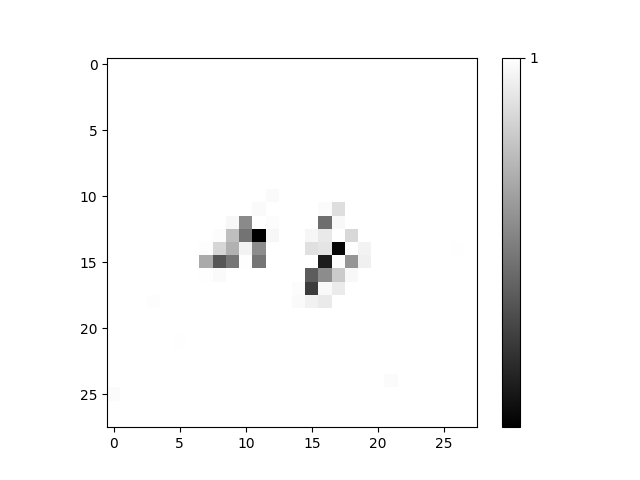
\includegraphics[width=\textwidth]{AND(LSM)/Positive/Layer0-Neuron-4.png}
		\caption{Digit 4}
	\end{minipage}
	\begin{minipage}[b]{0.19\textwidth}
		\captionsetup{labelformat=empty}
		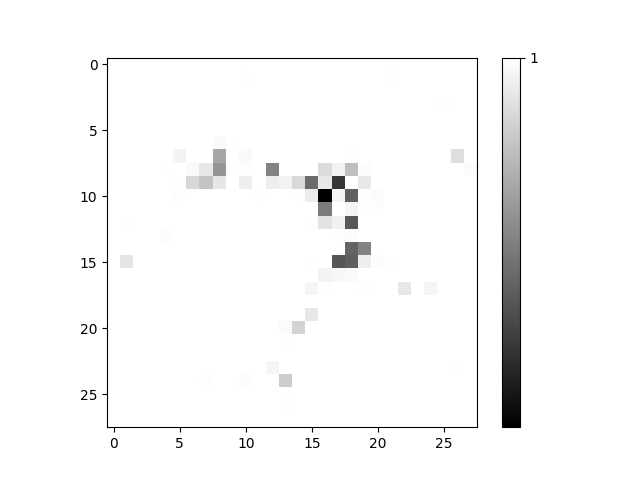
\includegraphics[width=\textwidth]{AND(LSM)/Positive/Layer0-Neuron-7.png}
		\caption{Digit 7}
	\end{minipage}
	\begin{minipage}[b]{0.19\textwidth}
		\captionsetup{labelformat=empty}
		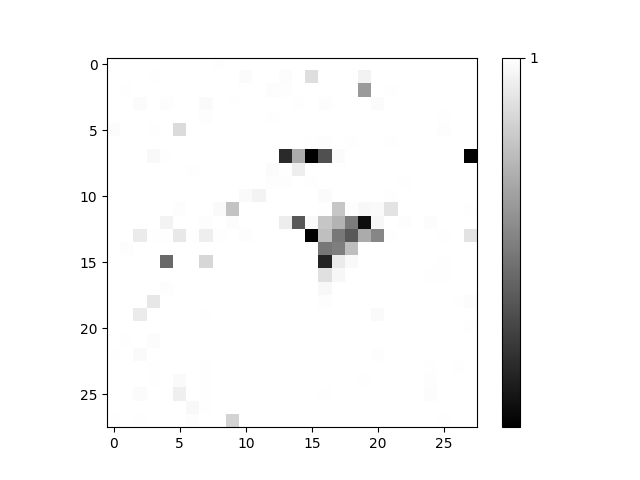
\includegraphics[width=\textwidth]{AND(LSM)/Positive/Layer0-Neuron-9.png}
		\caption{Digit 9}
	\end{minipage}
	\hfill
	\begin{minipage}[b]{0.19\textwidth}
		\captionsetup{labelformat=empty}
		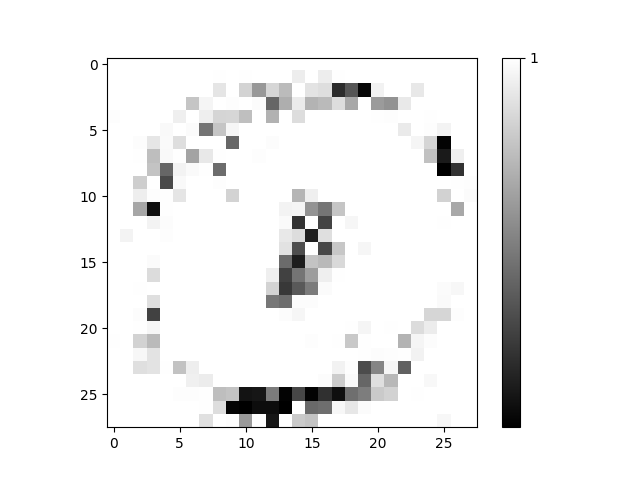
\includegraphics[width=\textwidth]{AND(LSM)/Negative/Layer0-Neuron-0.png}
		\caption{Not Digit 0}
	\end{minipage}
	\begin{minipage}[b]{0.19\textwidth}
		\captionsetup{labelformat=empty}
		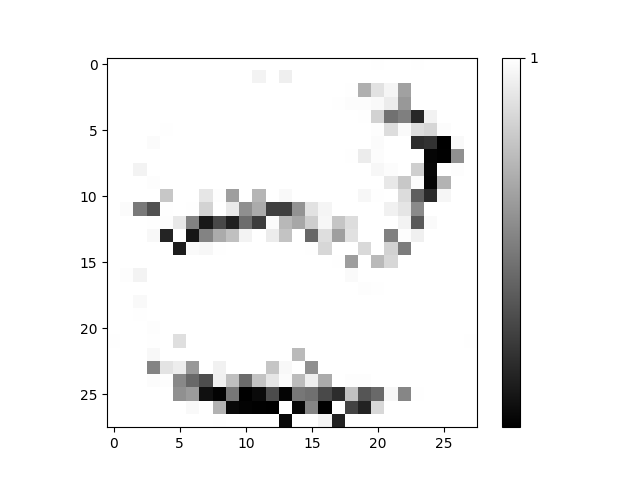
\includegraphics[width=\textwidth]{AND(LSM)/Negative/Layer0-Neuron-2.png}
		\caption{Not Digit 2}
	\end{minipage}
	\begin{minipage}[b]{0.19\textwidth}
		\captionsetup{labelformat=empty}
		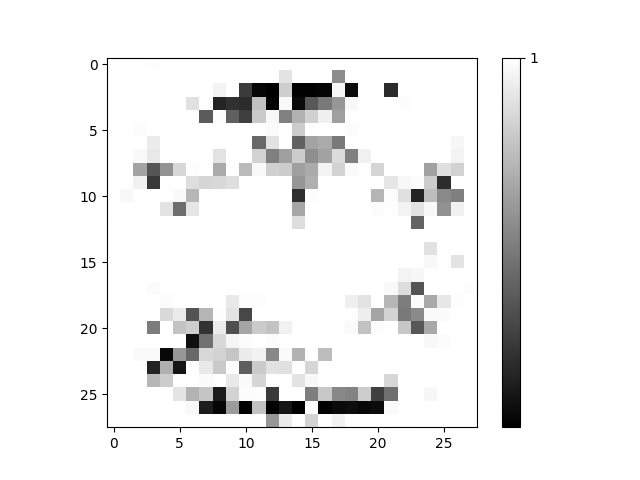
\includegraphics[width=\textwidth]{AND(LSM)/Negative/Layer0-Neuron-4.png}
		\caption{Not Digit 4}
	\end{minipage}
	\begin{minipage}[b]{0.19\textwidth}
		\captionsetup{labelformat=empty}
		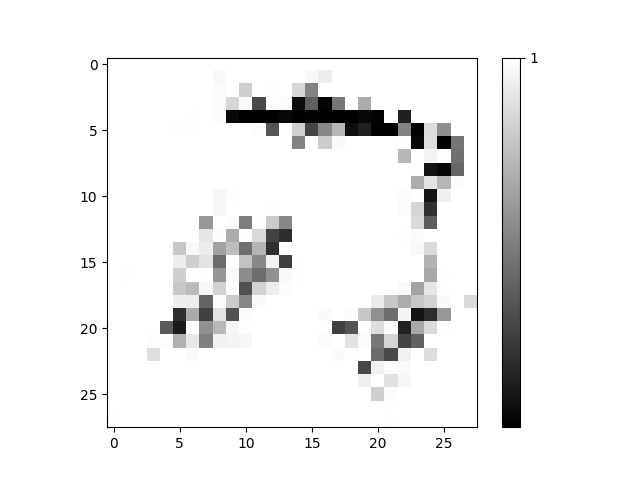
\includegraphics[width=\textwidth]{AND(LSM)/Negative/Layer0-Neuron-7.png}
		\caption{Not Digit 7}
	\end{minipage}
	\begin{minipage}[b]{0.19\textwidth}
		\captionsetup{labelformat=empty}
		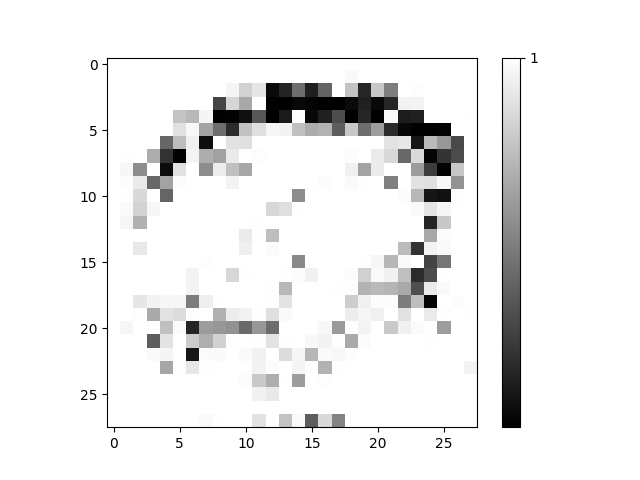
\includegraphics[width=\textwidth]{AND(LSM)/Negative/Layer0-Neuron-9.png}
		\caption{Not Digit 9}
	\end{minipage}
	\hfill
	\caption{Figures representing the weighted connections between the inputs and outputs for an AND network with an LSM. The top and bottom rows represent the positive/negative contributions retrespectively.}
	\label{fig:and-net-new-archetchure-with-lsm-interp}
\end{figure}

\paragraph{AND Network (With out LSM)}
Figure {} shows the positive/negative contributions to classification of the digits 0, 2, 4, 7 and 9. These features display the same patterns as the AND model with an LSM (Figure \ref{fig:and-net-new-archetchure-with-lsm-interp}) however the representations here are less noisy and have harder boundaries.

\begin{figure}[H]
	%\captionsetup{labelformat=empty}
	\centering
	\begin{minipage}[b]{0.19\textwidth}
		\captionsetup{labelformat=empty}
		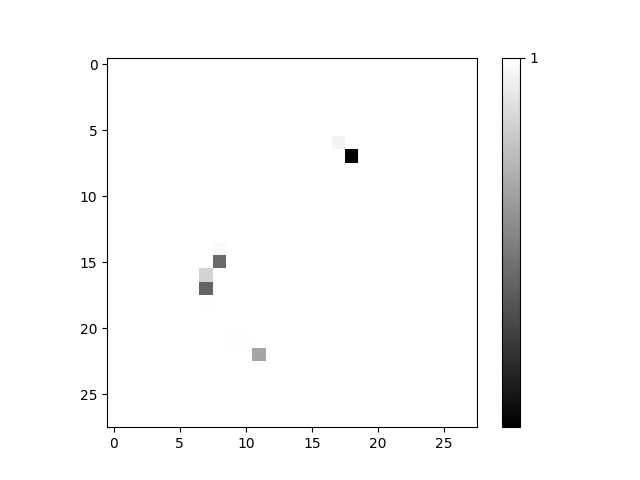
\includegraphics[width=\textwidth]{AND(NO-LSM)/Positive/Layer0-Neuron-0.png}
		\caption{Digit 0}
		\label{fig:cnf-descrete-generalizatiion}
	\end{minipage}
	\begin{minipage}[b]{0.19\textwidth}
		\captionsetup{labelformat=empty}
		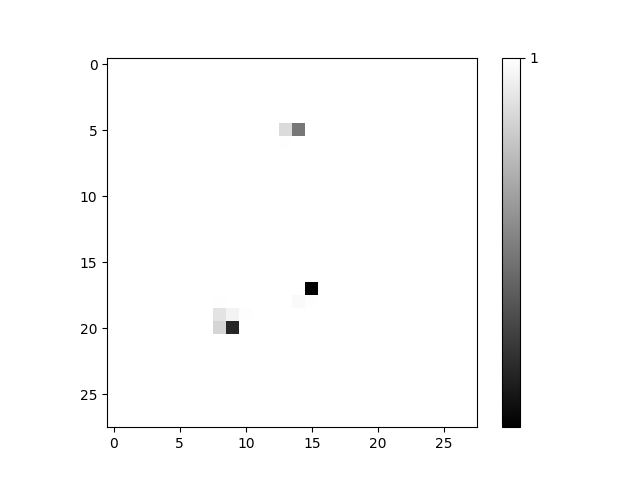
\includegraphics[width=\textwidth]{AND(NO-LSM)/Positive/Layer0-Neuron-2.png}
		\caption{Digit 2}
		\label{fig:cnf-descrete-generalizatiion}
	\end{minipage}
	\begin{minipage}[b]{0.19\textwidth}
		\captionsetup{labelformat=empty}
		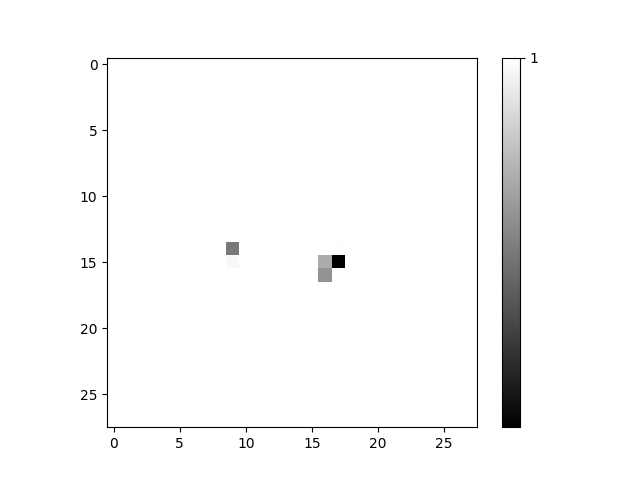
\includegraphics[width=\textwidth]{AND(NO-LSM)/Positive/Layer0-Neuron-4.png}
		\caption{Digit 4}
		\label{fig:cnf-descrete-generalizatiion}
	\end{minipage}
	\begin{minipage}[b]{0.19\textwidth}
		\captionsetup{labelformat=empty}
		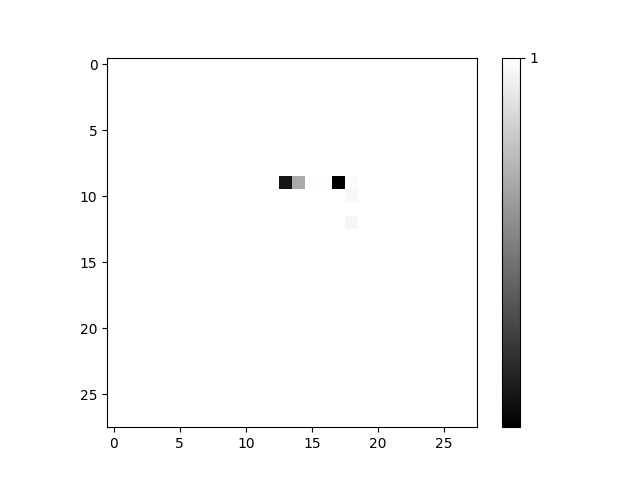
\includegraphics[width=\textwidth]{AND(NO-LSM)/Positive/Layer0-Neuron-7.png}
		\caption{Digit 7}
		\label{fig:cnf-descrete-generalizatiion}
	\end{minipage}
	\begin{minipage}[b]{0.19\textwidth}
		\captionsetup{labelformat=empty}
		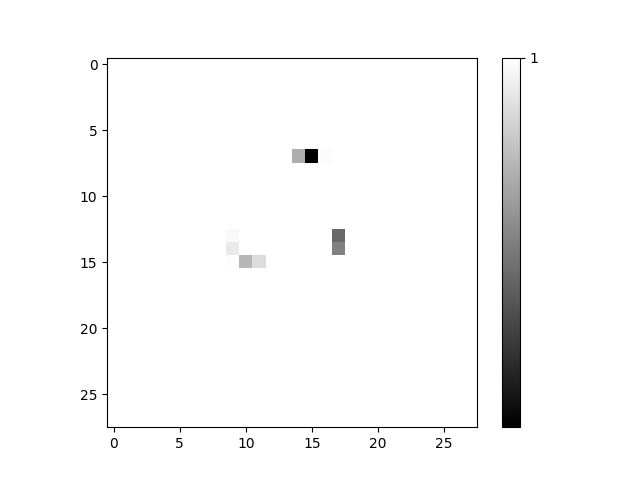
\includegraphics[width=\textwidth]{AND(NO-LSM)/Positive/Layer0-Neuron-9.png}
		\caption{Digit 9}
		\label{fig:cnf-descrete-generalizatiion}
	\end{minipage}
	\begin{minipage}[b]{0.19\textwidth}
		\captionsetup{labelformat=empty}
		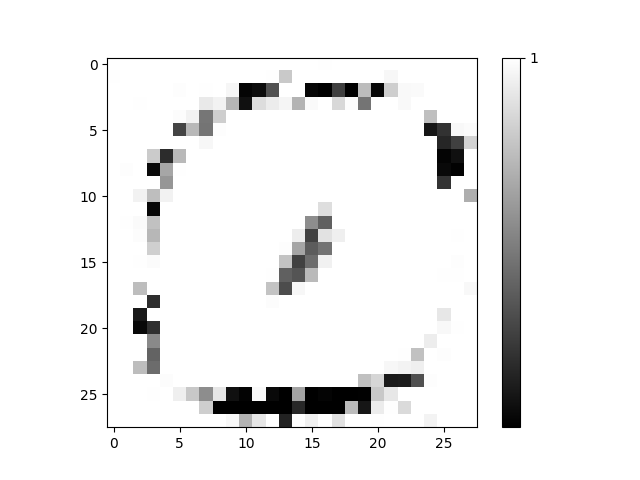
\includegraphics[width=\textwidth]{AND(NO-LSM)/Negative/Layer0-Neuron-0.png}
		\caption{Not Digit 0}
		\label{fig:cnf-descrete-generalizatiion}
	\end{minipage}
	\begin{minipage}[b]{0.19\textwidth}
		\captionsetup{labelformat=empty}
		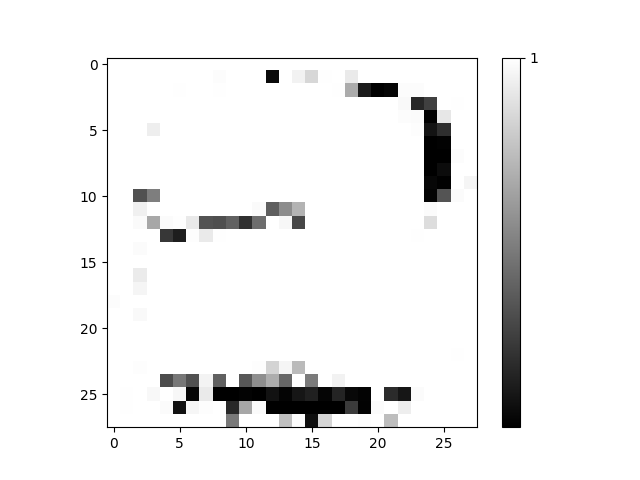
\includegraphics[width=\textwidth]{AND(NO-LSM)/Negative/Layer0-Neuron-2.png}
		\caption{Not Digit 2}
		\label{fig:cnf-descrete-generalizatiion}
	\end{minipage}
	\begin{minipage}[b]{0.19\textwidth}
		\captionsetup{labelformat=empty}
		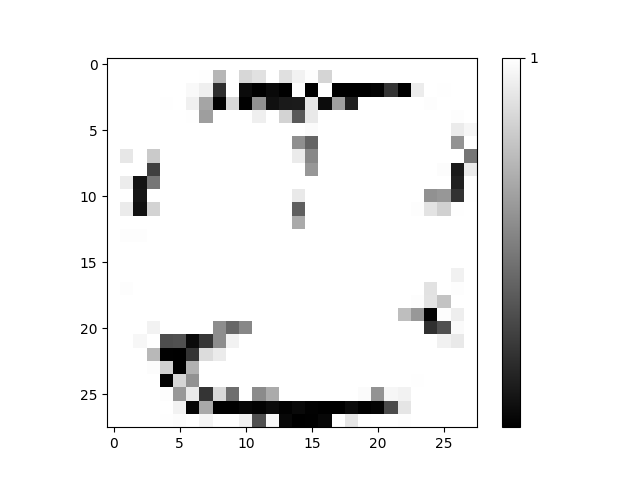
\includegraphics[width=\textwidth]{AND(NO-LSM)/Negative/Layer0-Neuron-4.png}
		\caption{Not Digit 4}
		\label{fig:cnf-descrete-generalizatiion}
	\end{minipage}
	\begin{minipage}[b]{0.19\textwidth}
		\captionsetup{labelformat=empty}
		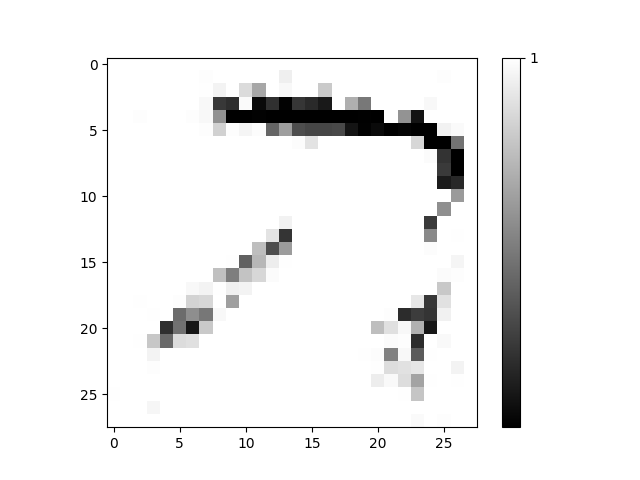
\includegraphics[width=\textwidth]{AND(NO-LSM)/Negative/Layer0-Neuron-7.png}
		\caption{Not Digit 7}
		\label{fig:cnf-descrete-generalizatiion}
	\end{minipage}
	\begin{minipage}[b]{0.19\textwidth}
		\captionsetup{labelformat=empty}
		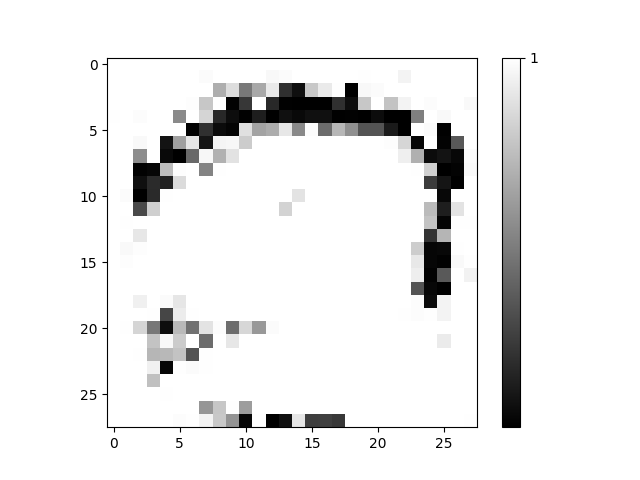
\includegraphics[width=\textwidth]{AND(NO-LSM)/Negative/Layer0-Neuron-9.png}
		\caption{Not Digit 9}
		\label{fig:cnf-descrete-generalizatiion}
	\end{minipage}
	\hfill
\end{figure}

\paragraph{Conclusion of Intepretability for LNNs with No Hidden Layer}
The logical Softmax introduces more noise into the weights but does not diminish the intepretability of the system. Using the new structure (i.e. adding nots of inputs) appears to change the means of which the LNN classifies the digits. Without NOTs the network positively weight the pixels which make-up the filling of the digits. On the other hand when the nots are added the network negatively weights pixels sitting just outside the border of the average digit.\\

Compared to the Sigmoid network the LNNs are more interpretable as it is possible to make determinations about how the network is making its classification decisions. These experements provide strong evidence in favour of the conclusion that LNNs with no hidden layers using new LNN architecture and LSM improve the intepretability when compared to MLPNs and old structure LNNs.

\subsubsection{Single Hidden Layer Networks}

Interpreting these multilayer models is a more difficult task as the hidden layer introduces dependencies between the inputs when considering how they influence the classification. To test the intepretability of these networks assume the goal is to verify that the digit 1 is being classified in a sensible way. With each network the hidden neurons which have the most influence on the classification be 1 will be displayed along with the ones which influence the classification not being 1.

\paragraph{Sigmoid Network}
The hidden features learnt by the Sigmoid Network do not appear to represent any meaningful information about the digit 1.

\begin{figure}[H]
	\centering
	\begin{minipage}[b]{0.19\textwidth}
		\captionsetup{labelformat=empty}
		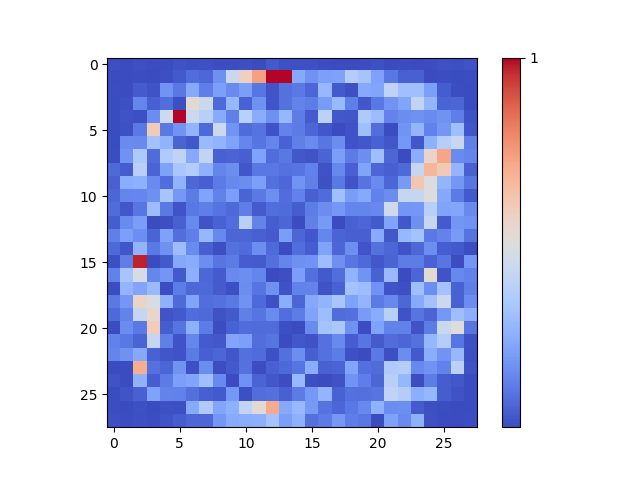
\includegraphics[width=\textwidth]{Sigmoid(Hidden-Layer)/Layer0-Neuron-6.png}
		%\caption{Digit 0}
		\label{}
	\end{minipage}
	\begin{minipage}[b]{0.19\textwidth}
		\captionsetup{labelformat=empty}
		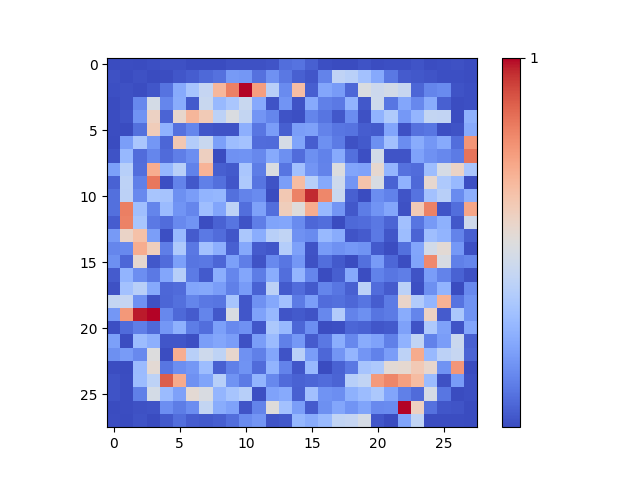
\includegraphics[width=\textwidth]{Sigmoid(Hidden-Layer)/Layer0-Neuron-7.png}
		%\caption{Digit 0}
		\label{}
	\end{minipage}
	\begin{minipage}[b]{0.19\textwidth}
		\captionsetup{labelformat=empty}
		\includegraphics[width=\textwidth]{Sigmoid(Hidden-Layer)/Layer0-Neuron-24.png}
		%\caption{Digit 0}
		\label{}
	\end{minipage}
	\begin{minipage}[b]{0.19\textwidth}
		\captionsetup{labelformat=empty}
		\includegraphics[width=\textwidth]{Sigmoid(Hidden-Layer)/Layer0-Neuron-28.png}
		%\caption{Digit 0}
		\label{}
	\end{minipage}
	\caption{}
	\hfill
\end{figure}

\paragraph{OR $\rightarrow$ AND Network Old Structure (With Out LSM)}
It is not immedatily apparent how the features in Figure \ref{fig:or-and-net-old-with-out-lsm} make up the digit 1. Each hidden feature is an OR of its inputs, as such only one of the dark pixles needs to be active for the neuron to be on. The first and last could be the stem of the 1 where as the middle one contains a dark bar at the bottom which could be the base.

\begin{figure}[H]
	%\captionsetup{labelformat=empty}
	\centering
	\begin{minipage}[b]{0.19\textwidth}
		\captionsetup{labelformat=empty}
		\includegraphics[width=\textwidth]{OR-AND(OLD)(WO-LSM)(1)/Layer0-Neuron-5.png}
		%\caption{Digit 0}
		\label{}
	\end{minipage}
	\begin{minipage}[b]{0.19\textwidth}
		\captionsetup{labelformat=empty}
		\includegraphics[width=\textwidth]{OR-AND(OLD)(WO-LSM)(1)/Layer0-Neuron-15.png}
		%\caption{Digit 0}
		\label{}
	\end{minipage}
	\begin{minipage}[b]{0.19\textwidth}
		\captionsetup{labelformat=empty}
		\includegraphics[width=\textwidth]{OR-AND(OLD)(WO-LSM)(1)/Layer0-Neuron-23.png}
		%\caption{Digit 0}
		\label{}
	\end{minipage}
	\caption{Features positively contributing to classification as a 1 for the OR $\rightarrow$ AND Network}
	\label{fig:or-and-net-old-with-out-lsm}
	\hfill
\end{figure}

\paragraph{OR $\rightarrow$ AND Network Old Structure (With LSM)}
In a similar fashion of the OR AND Network without an LSM these features are not clearly representative of a 1. Interestingly these weighting maps show that the features generally do not place a lot of emphasis on any particular inputs.
\begin{figure}[H]
	%\captionsetup{labelformat=empty}
	\centering
	\begin{minipage}[b]{0.19\textwidth}
		\captionsetup{labelformat=empty}
		\includegraphics[width=\textwidth]{OR-AND(OLD)(W-LSM)(1)/Layer0-Neuron-0.png}
		%\caption{Digit 0}
		\label{}
	\end{minipage}
	\begin{minipage}[b]{0.19\textwidth}
		\captionsetup{labelformat=empty}
		\includegraphics[width=\textwidth]{OR-AND(OLD)(W-LSM)(1)/Layer0-Neuron-2.png}
		%\caption{Digit 0}
		\label{}
	\end{minipage}
	\begin{minipage}[b]{0.19\textwidth}
		\captionsetup{labelformat=empty}
		\includegraphics[width=\textwidth]{OR-AND(OLD)(W-LSM)(1)/Layer0-Neuron-6.png}
		%\caption{Digit 0}
		\label{}
	\end{minipage}
	\begin{minipage}[b]{0.19\textwidth}
		\captionsetup{labelformat=empty}
	\includegraphics[width=\textwidth]{OR-AND(OLD)(W-LSM)(1)/Layer0-Neuron-7.png}
	%\caption{Digit 0}
	\label{}
	\end{minipage}
	\begin{minipage}[b]{0.19\textwidth}
		\captionsetup{labelformat=empty}
		\includegraphics[width=\textwidth]{OR-AND(OLD)(W-LSM)(1)/Layer0-Neuron-10.png}
		%\caption{Digit 0}
		\label{}
	\end{minipage}
	\begin{minipage}[b]{0.19\textwidth}
		\captionsetup{labelformat=empty}
		\includegraphics[width=\textwidth]{OR-AND(OLD)(W-LSM)(1)/Layer0-Neuron-14.png}
		%\caption{Digit 0}
		\label{}
	\end{minipage}
		\begin{minipage}[b]{0.19\textwidth}
		\captionsetup{labelformat=empty}
		\includegraphics[width=\textwidth]{OR-AND(OLD)(W-LSM)(1)/Layer0-Neuron-20.png}
		%\caption{Digit 0}
		\label{}
	\end{minipage}
	\begin{minipage}[b]{0.19\textwidth}
		\captionsetup{labelformat=empty}
		\includegraphics[width=\textwidth]{OR-AND(OLD)(W-LSM)(1)/Layer0-Neuron-29.png}
		%\caption{Digit 0}
		\label{}
	\end{minipage}

	\caption{Features positively contributing to the classification of 1 for the OR $\rightarrow$ AND Network Old Structure (With LSM)}
	\hfill
\end{figure}

\paragraph{OR $\rightarrow$ AND Network (With Out LSM)}
This network is running on the new architecture and as such each feature has two "channels". One representing the inputs that the feature positively likes and the other the inputs which are negatively liked (i.e. neuron is more active when these inputs are not present). The images in Figure \ref{fig:or-and-net-without-lsm-pos} represent the hidden features which if present contribute to the classification being the digit 1. These features are sparse and place a high weight on the inputs which they like.

\begin{figure}[H]
	%\captionsetup{labelformat=empty}
	\centering
	\begin{minipage}[b]{0.19\textwidth}
		\captionsetup{labelformat=empty}
		\includegraphics[width=\textwidth]{OR-AND(WO-LSM)(1)/Like/True/Layer0-Neuron-0.png}
		%\caption{Digit 0}
		\label{}
	\end{minipage}
	\begin{minipage}[b]{0.19\textwidth}
		\captionsetup{labelformat=empty}
		\includegraphics[width=\textwidth]{OR-AND(WO-LSM)(1)/Like/True/Layer0-Neuron-3.png}
		%\caption{Digit 0}
		\label{}
	\end{minipage}
	\begin{minipage}[b]{0.19\textwidth}
		\captionsetup{labelformat=empty}
		\includegraphics[width=\textwidth]{OR-AND(WO-LSM)(1)/Like/True/Layer0-Neuron-10.png}
		%\caption{Digit 0}
		\label{}
	\end{minipage}
	\begin{minipage}[b]{0.19\textwidth}
		\captionsetup{labelformat=empty}
		\includegraphics[width=\textwidth]{OR-AND(WO-LSM)(1)/Like/True/Layer0-Neuron-15.png}
		%\caption{Digit 0}
		\label{}
	\end{minipage}

	\medskip

		\begin{minipage}[b]{0.19\textwidth}
		\captionsetup{labelformat=empty}
		\includegraphics[width=\textwidth]{OR-AND(WO-LSM)(1)/Like/False/Layer0-Neuron-0.png}
		%\caption{Digit 0}
		\label{}
	\end{minipage}
	\begin{minipage}[b]{0.19\textwidth}
		\captionsetup{labelformat=empty}
		\includegraphics[width=\textwidth]{OR-AND(WO-LSM)(1)/Like/False/Layer0-Neuron-3.png}
		%\caption{Digit 0}
		\label{}
	\end{minipage}
	\begin{minipage}[b]{0.19\textwidth}
		\captionsetup{labelformat=empty}
		\includegraphics[width=\textwidth]{OR-AND(WO-LSM)(1)/Like/False/Layer0-Neuron-10.png}
		%\caption{Digit 0}
		\label{}
	\end{minipage}
	\begin{minipage}[b]{0.19\textwidth}
		\captionsetup{labelformat=empty}
		\includegraphics[width=\textwidth]{OR-AND(WO-LSM)(1)/Like/False/Layer0-Neuron-15.png}
		%\caption{Digit 0}
		\label{}
	\end{minipage}
	\caption{Features positively contributing to classification as a 1 for OR $\rightarrow$ AND Network (With Out LSM)}
	\label{fig:or-and-net-without-lsm-pos}
	\hfill
\end{figure}


\begin{figure}[H]
	\begin{minipage}[t]{0.44\textwidth}
		\vspace{0cm}
		It is not immediatly obvious what the features showin in Figure \ref{fig:or-and-net-without-lsm-pos} represent. Figure \ref{fig:or-and-net-without-lsm-neg} shows the single feature which if present then the classification is less likely to be the digit 1. This feature appears to be highley active if the pixles lieing outside an area which looks like the average 1 shape.\\

		While this model is diffcult to intepret it does provide more information than previous OR AND models using the old LNN archetchure.
	\end{minipage}
	\hspace{1cm}
	\begin{minipage}[t]{0.49\textwidth}
	\vspace{0cm}
	%\captionsetup{labelformat=empty}
	\centering
	\begin{minipage}[b]{0.49\textwidth}
		\captionsetup{labelformat=empty}
		\includegraphics[width=\textwidth]{OR-AND(WO-LSM)(1)/DontLike/True/Layer0-Neuron-28.png}
		%\caption{Digit 0}
		\label{}
	\end{minipage}

	\medskip

	\begin{minipage}[b]{0.49\textwidth}
		\captionsetup{labelformat=empty}
		\includegraphics[width=\textwidth]{OR-AND(WO-LSM)(1)/DontLike/False/Layer0-Neuron-28.png}
		%\caption{Digit 0}
		\label{}
	\end{minipage}
	\caption{Features contributing to classification not being 1 for OR $\rightarrow$ AND Network (With Out LSM)}
	\label{fig:or-and-net-without-lsm-neg}
	\hfill
	\end{minipage}
\end{figure}

\begin{figure}[H]
	%\captionsetup{labelformat=empty}
	\centering
	\begin{minipage}[t]{0.44\textwidth}
		\vspace{0.2cm}
		\paragraph{OR $\rightarrow$ AND (With LSM)} Figure \ref{fig:or-and-with-lsm-pos} show the positive features for an OR AND model with an LSM. 
The features extracted from this network do not appear to correspond to a 1, not in a way which is immediately interpretable. 
	\end{minipage}
	\hspace{1cm}
	\begin{minipage}[t]{0.44\textwidth}
		\vspace{0cm}
		\begin{minipage}[b]{0.49\textwidth}
		\captionsetup{labelformat=empty}
		\includegraphics[width=\textwidth]{OR-AND(W-LSM)(1)/Like/True/Layer0-Neuron-18.png}
		%\caption{Digit 0}
		\label{}
	\end{minipage}
	\begin{minipage}[b]{0.49\textwidth}
		\captionsetup{labelformat=empty}
		\includegraphics[width=\textwidth]{OR-AND(W-LSM)(1)/Like/True/Layer0-Neuron-19.png}
		%\caption{Digit 0}
		\label{}
	\end{minipage}
	
	\medskip
	
	\begin{minipage}[b]{0.49\textwidth}
		\captionsetup{labelformat=empty}
		\includegraphics[width=\textwidth]{OR-AND(W-LSM)(1)/Like/False/Layer0-Neuron-18.png}
		%\caption{Digit 0}
		\label{}
	\end{minipage}
	\begin{minipage}[b]{0.49\textwidth}
		\captionsetup{labelformat=empty}
		\includegraphics[width=\textwidth]{OR-AND(W-LSM)(1)/Like/False/Layer0-Neuron-19.png}
		%\caption{Digit 0}
		\label{}
	\end{minipage}
	\caption{Features positively contributing to the classification being 1 for OR $\rightarrow$ AND (With LSM)}		
	\label{fig:or-and-with-lsm-pos}
	\end{minipage}
	\hfill
\end{figure}

The following features are the ones which are negatively weighted towards being a 1. 

\begin{figure}[H]

	%\captionsetup{labelformat=empty}
	\centering
	\begin{minipage}[b]{0.19\textwidth}
		\captionsetup{labelformat=empty}
		\includegraphics[width=\textwidth]{OR-AND(W-LSM)(1)/DontLike/True/Layer0-Neuron-2.png}
		%\caption{Digit 0}
		\label{}
	\end{minipage}
	\begin{minipage}[b]{0.19\textwidth}
		\captionsetup{labelformat=empty}
		\includegraphics[width=\textwidth]{OR-AND(W-LSM)(1)/DontLike/True/Layer0-Neuron-9.png}
		%\caption{Digit 0}
		\label{}
	\end{minipage}
	\begin{minipage}[b]{0.19\textwidth}
		\captionsetup{labelformat=empty}
		\includegraphics[width=\textwidth]{OR-AND(W-LSM)(1)/DontLike/True/Layer0-Neuron-28.png}
		%\caption{Digit 0}
		\label{}
	\end{minipage}
	
	\medskip
	
	\begin{minipage}[b]{0.19\textwidth}
		\captionsetup{labelformat=empty}
	\includegraphics[width=\textwidth]{OR-AND(W-LSM)(1)/DontLike/False/Layer0-Neuron-2.png}
	%\caption{Digit 0}
	\label{}
\end{minipage}
\begin{minipage}[b]{0.19\textwidth}
		\captionsetup{labelformat=empty}
	\includegraphics[width=\textwidth]{OR-AND(W-LSM)(1)/DontLike/False/Layer0-Neuron-9.png}
	%\caption{Digit 0}
	\label{}
\end{minipage}
\begin{minipage}[b]{0.19\textwidth}
		\captionsetup{labelformat=empty}
	\includegraphics[width=\textwidth]{OR-AND(W-LSM)(1)/DontLike/False/Layer0-Neuron-28.png}
	%\caption{Digit 0}
	\label{}
\end{minipage}
	\caption{Features contributing to the classification not being 1 for OR $\rightarrow$ AND (With LSM)}
	\hfill
\end{figure}
\begin{figure}[H]
	\begin{minipage}[t]{0.48\textwidth}
		\vspace{0px}
		\paragraph{AND $\rightarrow$ OR Model (With Out LSM)}
This network has a small number of features associated with each classification. In terms of the classifying the digit 1 there is only 1 hidden features. This feature appears to classify a 1 by positively liking the stem of a 1 and disliking the anything outside the average 1.\\ \\

		\paragraph{AND $\rightarrow$ OR Model (With LSM)}
Similarly to the AND OR Model with out the LSM this model appears to positively like the inputs on the stem of a 1 and dislike any pixel outside the average border of a 1.
	\end{minipage}
	\hspace{2px}
	\begin{minipage}[t]{0.44\textwidth}
	\vspace{0px}
			%\captionsetup{labelformat=empty}
	\centering
	\begin{minipage}[b]{0.5\textwidth}
		\captionsetup{labelformat=empty}
		\includegraphics[width=\textwidth]{AND-OR(WO-LSM)(1)/Like/True/Layer0-Neuron-3.png}
		%\caption{Digit 0}
		\label{}
	\end{minipage}
	
	\medskip

	\begin{minipage}[b]{0.5\textwidth}
		\captionsetup{labelformat=empty}
		\includegraphics[width=\textwidth]{AND-OR(WO-LSM)(1)/Like/False/Layer0-Neuron-3.png}
		%\caption{Digit 0}
		\label{}
	\end{minipage}
	\caption{Features positively contributing to classification as 1 for AND $\rightarrow$ OR Model (With Out LSM)}
	\end{minipage}

	\hfill
\end{figure}

\begin{figure}[H]
	\begin{minipage}[t]{0.48\textwidth}
		\vspace{0px}
		\paragraph{Conclusion of Intepretability for LNNs with No Hidden Layer}
The results of the experiments show that in the context of multi layer adding an LSM introduces more noise into the feature maps. And similarly to before the sigmoid weights do not appear to relate to digit 1 in any meaningful way.
	\end{minipage}
\hspace{2px}
	\begin{minipage}[t]{0.5\textwidth}
\vspace{0px}
			%\captionsetup{labelformat=empty}
	\centering
	\begin{minipage}[b]{0.5\textwidth}
		\captionsetup{labelformat=empty}
		\includegraphics[width=\textwidth]{AND-OR(W-LSM)(1)/Like/True/Layer0-Neuron-9.png}
		%\caption{Digit 0}
		\label{}
	\end{minipage}
	
	\medskip
	
	\begin{minipage}[b]{0.5\textwidth}
		\captionsetup{labelformat=empty}
		\includegraphics[width=\textwidth]{AND-OR(W-LSM)(1)/Like/False/Layer0-Neuron-9.png}
		%\caption{Digit 0}
		\label{}
	\end{minipage}
	\caption{Features contributing to classification not being 1 for AND $\rightarrow$ OR Model (With Out LSM)}
	\end{minipage}
	\hfill
\end{figure}

\subsection{Comparason between LNN Intepretability and LIME}
The aim of LIME is to build trust in the model by explaining how a specific predictions are arrived at.  Whereas LNN intepretability comes down to directly identifying what input features contribute to each output neuron being active. The LIME algorythm will be used to intepret an MLPN and LNN. It is able to determin 


\subsection{Results of Intepretability Experiments}
From the above experiments and discussions the following conclusions can be made

\begin{enumerate}
	\item \textit{Rules Extracted are Intepretable:} The Tic-Tac-Toe problem experiments showed that the rules extracted from LNNs where intepretable.
	\item \textit{Adding Nots Improves Intepretability:} Using the new structure with nots allows the network to place a greater emphasis on the presence or absence of various pixels. Without the Nots not many of inputs are of great importance, rather many have a relatively small relevance.
	\item \textit{Adding an Logical Soft Max does not hinder the intepretability (on the new architecture):} By comparing the two different network architectures with and without an LSM it is possible to see that the intepretability is not directly effected and the features representing the classification of the digit 1 are not significantly changed.
	\item \textit{Intepretability of Network is Heavily Dependent on Structure:} As shown through the previous examples the OR $\rightarrow$ AND networks harder to interpret than the AND $\rightarrow$ OR architecture.
\end{enumerate}

\section{Summary Of Logical Neural Network Evaluation}
Through the experiments carried out the following observations can be made.

\begin{enumerate}
	\item \textit{Performance comparison between the old and new Logical Neural Network Structures:} The new LNN structure (adding NOTs) results with a statistically significant increase in accuracy with some network architectures.
	\item \textit{Performance comparison between Multi Layer Perceptron Network and new LNNs:} The new LNN structure achieved statistically equivalent or better performance than the MLPN nets with an equivalent number of hidden neurons/layers.
	\item \textit{Performance comparison between networks with and without Logical Softmax:} For any LNN (new structure or old) adding a Logical Softmax improved performance by a statistically significant margin.
	\item \textit{Comparison of intepretability between MLPNs and new/old LNNs:} Any LNN (new or old structure) was more interpretable than the corresponding MLPN.
	\item \textit{Comparison of intepretability between MLPNs (using LIME) and new/old LNNs:}
\end{enumerate}

These experiments have therefore provided evidence demonstrating that the modified LNN structure and logical softmax improves upon the current state of LNNs.  

\chapter{Application to Auto Encoders} \label{C:lnn-application}
This chapter demonstraits the flexability of the LNN archecthure by applying them in the context of Auto Encoders. \\

Auto encoders \cite{baldi2012complex} \hl{are a network architecture trained with unsupervised learning for a purpose of learning an encoding of the data}. \hl{An application learning a new encoding is dimensionality reduction}. The aim is to take the input to some reduced feature space and then from this feature space back to the original input with the smallest error. The case where there is one linear layer doing the encoding and decoding is called \textbf{Linear Autoencoder}, this architecture corresponds to performing Principle Component Analysis (PCA) on the data.\\

\hl{For some data sets, such as MNIST, PCA is not an effective way to reduce the dimensions of the data}. For this reason Logical Autoencoders are proposed (Definition \ref{def:logical-autoencoder}) as an alternative means to lower the dimensions of a dataset.

\begin{definition} \label{def:logical-autoencoder}
	A \textbf{Logical Autoencoder} is an Autoencoder where the encoder and decoder are LNNs
\end{definition}

The experiments carried out will be to compress the MNIST feature space (784 dimensions) into 10 dimensions using different Auto encoder architectures. The accuracy and intepretability of the features will be explored. Each model was trained for 30 epochs

\paragraph{Result of Logical Auto Encoder (LoAE)}
A logical auto encoder, consisting of a single AND layer for both the encoder and decoder, was able to compress the feature space to 20 dimensions and achieve a Mean Square Error (MSE) of 20.55 on the training set and 20.22 on the testing set.

\begin{figure}[H]
	%\captionsetup{labelformat=empty}
	\centering
	\begin{minipage}[b]{0.19\textwidth}
		\captionsetup{labelformat=empty}
		\includegraphics[width=\textwidth]{LoAE(AND)(20LF)/True/Feature-0.png}
		%\caption{Digit 0}
		\label{}
	\end{minipage}
	\begin{minipage}[b]{0.19\textwidth}
		\captionsetup{labelformat=empty}
		\includegraphics[width=\textwidth]{LoAE(AND)(20LF)/True/Feature-4.png}
		%\caption{Digit 0}
		\label{}
	\end{minipage}
	\begin{minipage}[b]{0.19\textwidth}
		\captionsetup{labelformat=empty}
		\includegraphics[width=\textwidth]{LoAE(AND)(20LF)/True/Feature-10.png}
		%\caption{Digit 0}
		\label{}
	\end{minipage}
	\begin{minipage}[b]{0.19\textwidth}
		\captionsetup{labelformat=empty}
		\includegraphics[width=\textwidth]{LoAE(AND)(20LF)/True/Feature-12.png}
		%\caption{Digit 0}
		\label{}
	\end{minipage}
	\begin{minipage}[b]{0.19\textwidth}
		\captionsetup{labelformat=empty}
		\includegraphics[width=\textwidth]{LoAE(AND)(20LF)/True/Feature-17.png}
		%\caption{Digit 0}
		\label{}
	\end{minipage}
	
	\medskip
	
		\begin{minipage}[b]{0.19\textwidth}
		\captionsetup{labelformat=empty}
		\includegraphics[width=\textwidth]{LoAE(AND)(20LF)/False/Feature-0.png}
		%\caption{Digit 0}
		\label{}
	\end{minipage}
	\begin{minipage}[b]{0.19\textwidth}
		\captionsetup{labelformat=empty}
		\includegraphics[width=\textwidth]{LoAE(AND)(20LF)/False/Feature-4.png}
		%\caption{Digit 0}
		\label{}
	\end{minipage}
	\begin{minipage}[b]{0.19\textwidth}
		\captionsetup{labelformat=empty}
		\includegraphics[width=\textwidth]{LoAE(AND)(20LF)/False/Feature-10.png}
		%\caption{Digit 0}
		\label{}
	\end{minipage}
	\begin{minipage}[b]{0.19\textwidth}
		\captionsetup{labelformat=empty}
		\includegraphics[width=\textwidth]{LoAE(AND)(20LF)/False/Feature-12.png}
		%\caption{Digit 0}
		\label{}
	\end{minipage}
	\begin{minipage}[b]{0.19\textwidth}
		\captionsetup{labelformat=empty}
		\includegraphics[width=\textwidth]{LoAE(AND)(20LF)/False/Feature-17.png}
		%\caption{Digit 0}
		\label{}
	\end{minipage}
	
	\hfill
\end{figure}

\comment{Re Compute images of features}
\paragraph{Result of Linear Auto Encoder (LAE)}
A linear auto encoder obtained an MSE of 21.34 on the training and 21.25 on the test data.

\begin{figure}[H]
	%\captionsetup{labelformat=empty}
	\centering
	\begin{minipage}[b]{0.19\textwidth}
		\captionsetup{labelformat=empty}
		\includegraphics[width=\textwidth]{Linear-AE/Feature-3.png}
		%\caption{Digit 0}
		\label{}
	\end{minipage}
	\begin{minipage}[b]{0.19\textwidth}
		\captionsetup{labelformat=empty}
		\includegraphics[width=\textwidth]{Linear-AE/Feature-7.png}
		%\caption{Digit 0}
		\label{}
	\end{minipage}
	\begin{minipage}[b]{0.19\textwidth}
		\captionsetup{labelformat=empty}
		\includegraphics[width=\textwidth]{Linear-AE/Feature-11.png}
		%\caption{Digit 0}
		\label{}
	\end{minipage}
	\begin{minipage}[b]{0.19\textwidth}
		\captionsetup{labelformat=empty}
		\includegraphics[width=\textwidth]{Linear-AE/Feature-15.png}
		%\caption{Digit 0}
		\label{}
	\end{minipage}
	\begin{minipage}[b]{0.19\textwidth}
		\captionsetup{labelformat=empty}
		\includegraphics[width=\textwidth]{Linear-AE/Feature-18.png}
		%\caption{Digit 0}
		\label{}
	\end{minipage}
	
	\hfill
\end{figure}

\paragraph{Result of Sigmoid Auto Encoder (SAE)}
A sigmoid Autoencoder achieved an MSE of 14.43 on the training data and 14.25 on the testing data.

\begin{figure}[H]
	%\captionsetup{labelformat=empty}
	\centering
	\begin{minipage}[b]{0.19\textwidth}
		\captionsetup{labelformat=empty}
		\includegraphics[width=\textwidth]{SAE(20LF)/Feature-0.png}
		%\caption{Digit 0}
		\label{}
	\end{minipage}
	\begin{minipage}[b]{0.19\textwidth}
		\captionsetup{labelformat=empty}
		\includegraphics[width=\textwidth]{SAE(20LF)/Feature-6.png}
		%\caption{Digit 0}
		\label{}
	\end{minipage}
	\begin{minipage}[b]{0.19\textwidth}
		\captionsetup{labelformat=empty}
		\includegraphics[width=\textwidth]{SAE(20LF)/Feature-10.png}
		%\caption{Digit 0}
		\label{}
	\end{minipage}
	\begin{minipage}[b]{0.19\textwidth}
		\captionsetup{labelformat=empty}
		\includegraphics[width=\textwidth]{SAE(20LF)/Feature-12.png}
		%\caption{Digit 0}
		\label{}
	\end{minipage}
	\begin{minipage}[b]{0.19\textwidth}
		\captionsetup{labelformat=empty}
		\includegraphics[width=\textwidth]{SAE(20LF)/Feature-15.png}
		%\caption{Digit 0}
		\label{}
	\end{minipage}
	
	\hfill
\end{figure}

\paragraph{Discussion}
While the results show that the Sigmoid Auto Encoder (AE) outperforms the Logical one this is an example of how Logical Neural Networks can be applied to different situations in Machine Learning where the goals are different from classification. The features learnt by the Logical AE are sparse and possible interpretable as each one can be viewed as a logical AND of the input features.\\

A Logical Auto Encoder provides a means to trade off between the intepretableity of the model and the performance.
